%! TEX program = xelatex
%%%%%%%%%%%%%%%%%%%%%%%%%%%%%%%%%%%%%%%%%%%%%%%%%%%%%%%%%%%%%%%%%%%%%%%%%%%%%%%%
% Preámbulo                                                                    %
%%%%%%%%%%%%%%%%%%%%%%%%%%%%%%%%%%%%%%%%%%%%%%%%%%%%%%%%%%%%%%%%%%%%%%%%%%%%%%%%

\documentclass[11pt,a4paper,titlepage,oneside]{report}

%%% RELACIÓN DE VARIABLES A PERSONALIZAR %%%
%\def\lingua{gal}
\def\lingua{esp} % descomenta esta liña se redactarás a memoria en español
%\def\lingua{eng} % descomenta esta liña se redactarás a memoria en inglés
\def\nome{Héctor Aldao Amoedo}                             % substitúe aquí o teu nome
\def\nomedirectorA{Alejeandro Rodrigez Árias}              % substitúe aquí o nome de quen dirixe
\def\nomedirectorB{Samuel Magaz Romero}             % duplica esta liña máis veces se o precisas, cambiando
                                                     % a letra final (A, B, C, D...): úsanse na portada.tex
\def\titulo{Visualizando el aprendizaje máquina: de la abstracción al entendimiento} % substitúe aquí o título do teu TFG
%\def\titulacion{gced}                               % descomenta esta liña e comenta a seguinte se es estudante do GCED
\def\titulacion{gia}
%\def\mencion{COMPUTACIÓN}                           % descomenta a mención que che corresponda se es estudante do GEI
%\def\mencion{ENXEÑARÍA DO SOFTWARE}
%\def\mencion{ENXEÑARÍA DE COMPUTADORES}
%\def\mencion{SISTEMAS DE INFORMACIÓN}
%\def\mencion{TECNOLOXÍAS DA INFORMACIÓN}

%\def\renomearcadros{si} % descomenta esta liña se redactas a memoria en español e prefires que
                         % os "cuadros" e o "índice de cuadros" se renomeen
                         % a "tablas" e "índice de tablas" respectivamente

\usepackage{estilo_tfg}

% Lista de paquetes potencialmente interesantes (uso baixo demanda)

% \usepackage{alltt}       % proporciona o entorno alltt, semellante a verbatim pero que respecta comandos
% \usepackage{enumitem}    % permite personalizar os entornos de lista
% \usepackage{eurofont}    % proporciona o comando \euro
\usepackage{float}       % permite máis opcións para controlar obxectos flotantes (táboas, figuras)
% \usepackage{hhline}      % permite personalizar as liñas horizontais en arrays e táboas
  \usepackage{longtable}   % permite construir táboas que ocupan máis dunha páxina
% \usepackage{lscape}      % permite colocar partes do documento en orientación apaisada
% \usepackage{moreverb}    % permite personalizar o entorno verbatim
% \usepackage{multirow}    % permite crear celdas que ocupan varias filas da mesma táboa
% \usepackage{pdfpages}    % permite insertar ficheiros en PDF no documento
% \usepackage{rotating}    % permite diferentes tipos de rotacións para figuras e táboas
% \usepackage{subcaption}  % permite a inclusión de varias subfiguras nunha figura
% \usepackage{tabu}        % permite táboas flexibles
% \usepackage{tabularx}    % permite táboas con columnas de anchura determinada

%%%%%%%%%%%%%%%%%%%%%%%%%%%%%%%%%%%%%%%%%%%%%%%%%%%%%%%%%%%%%%%%%%%%%%%%%%%%%%%%
% Corpo                                                                        %
%%%%%%%%%%%%%%%%%%%%%%%%%%%%%%%%%%%%%%%%%%%%%%%%%%%%%%%%%%%%%%%%%%%%%%%%%%%%%%%%

\begin{document}

 %%%%%%%%%%%%%%%%%%%%%%%%%%%%%%%%%%%%%%%%
 % Preliminares do documento            %
 %%%%%%%%%%%%%%%%%%%%%%%%%%%%%%%%%%%%%%%%

 \include{portada/portada}
 \dedicatoria{A Paulo González Ogando, mi profesor de matemáticas del instituto.
 Este es mi intento de explicar lo que he aprendido en esta carrera tan bien como él nos explicaba su asignatura.} % escribe neste comando o teu texto de dedicatoria
 \paxinaenbranco
 \begin{agradecementos}
 %\blindtext                % substitúe este comando polo teu texto de agradecementos
  A mi familia por el apollo infinito, a Bombardeen por la compañía y las risas, y a Las Damas por el tiempo y el cariño.
 \end{agradecementos}
 %%%%%%%%%%%%%%%%%%%%%%%%%%%%%%%%%%%%%%%%%%%%%%%%%%%%%%%%%%%%%%%%%%%%%%%%%%%%%%%%

\pagestyle{empty}
\begin{abstract}
  Los modelos de inteligencia artificial tienen una presencia cada vez mayor en ámbitos técnicos y cotidianos, aunque su funcionamiento interno puede resultar difícil de comprender cuando se estudia únicamente a través de fórmulas o código.
  En los modelos de aprendizaje automático, esta dificultad se acentúa porque el proceso depende de operaciones que no siempre son visibles para quien aprende o usa los algoritmos.
  Este trabajo presenta el diseño y desarrollo de una aplicación web educativa, implementada en Godot, para visualizar de forma interactiva el funcionamiento interno de dos modelos básicos de aprendizaje automático supervisado: los árboles de decisión y las redes neuronales multicapa.
  La herramienta está orientada a facilitar la comprensión intuitiva de estos procesos mediante la evolución paso a paso de los algoritmos, acompañando cada estado con explicaciones textuales y representaciones gráficas.

  En el módulo de árboles de decisión se implementa un algoritmo basado en ID3 para atributos categóricos.
  Durante el entrenamiento, el usuario puede observar cómo se seleccionan los atributos mediante una métrica basada en la entropía y cómo se crean los nodos y las ramas.
  La fase de evaluación representa el recorrido de nuevos ejemplos por el árbol ya entrenado hasta obtener su clasificación.
  En el módulo de redes neuronales se implementa un perceptrón multicapa configurable, con selección de datos, definición de arquitectura, ejecución del \textit{forward pass}, cálculo del error, retropropagación y actualización visual de pesos y sesgos.
  La aplicación incorpora ventanas informativas con fórmulas, gráficas de activación, carga de conjuntos de datos y persistencia de modelos.
  El resultado final se despliega como aplicación HTML5 mediante GitHub Pages, lo que permite acceder al recurso desde un navegador y utilizarlo como apoyo al aprendizaje de estos algoritmos.

  \vspace*{25pt}
  \begin{segundoresumo}
    Artificial intelligence models are increasingly present in technical and everyday contexts, although their internal behavior can be difficult to understand when it is studied only through formulas or code.
    In machine learning models, this difficulty becomes more pronounced because the process depends on operations that are not always visible to those who learn or use the algorithms.
    This work presents the design and development of an educational web application, implemented in Godot, for the interactive visualization of the internal behavior of two basic supervised machine learning models: decision trees and multilayer neural networks.
    The tool aims to support an intuitive understanding of these processes through the step-by-step evolution of the algorithms, linking each state with textual explanations and graphical representations.

    The decision tree module implements an ID3-based algorithm for categorical attributes.
    During training, the user can observe how attributes are selected through an entropy-based metric and how nodes and branches are created.
    The evaluation stage represents the path followed by new examples through the trained tree until a classification is obtained.
    The neural network module implements a configurable multilayer perceptron, with dataset selection, architecture definition, \textit{forward pass} execution, error calculation, backpropagation and visual updates of weights and biases.
    The application includes informative panels with formulas, activation graphs, dataset loading and model persistence.
    The final result is deployed as an HTML5 application through GitHub Pages, allowing the resource to be accessed from a browser and used as support for learning these algorithms.
  \end{segundoresumo}
\vspace*{25pt}
\begin{multicols}{2}
\begin{description}
\item [\palabraschaveprincipal:] \mbox{} \\[-20pt]
  \begin{itemize}
    \item Aprendizaje automático
    \item Aprendizaje supervisado
    \item Visualización interactiva
    \item Godot
    \item Árboles de decisión
    \item Redes neuronales multicapa
    \item Aplicaciones web educativas
  \end{itemize}
\end{description}
\begin{description}
\item [\palabraschavesecundaria:] \mbox{} \\[-20pt]
  \begin{itemize}
    \item Machine learning
    \item Supervised learning
    \item Interactive visualization
    \item Godot
    \item Decision trees
    \item Multilayer perceptrons
    \item Educational web applications
  \end{itemize}
\end{description}
\end{multicols}

\end{abstract}
\pagestyle{fancy}

%%%%%%%%%%%%%%%%%%%%%%%%%%%%%%%%%%%%%%%%%%%%%%%%%%%%%%%%%%%%%%%%%%%%%%%%%%%%%%%%


 \pagenumbering{roman}
 \setcounter{page}{1}
 \bstctlcite{IEEEexample:BSTcontrol}

 \tableofcontents
 \listoffigures
 \listoftables
 \clearpage
 
 \pagenumbering{arabic}
 \setcounter{page}{1}

 %%%%%%%%%%%%%%%%%%%%%%%%%%%%%%%%%%%%%%%%
 % Capítulos                            %
 %%%%%%%%%%%%%%%%%%%%%%%%%%%%%%%%%%%%%%%%

 \chapter{Introdución}
\label{chap:introducion}

\lettrine{L}{a} inteligencia artificial agrupa técnicas orientadas a construir sistemas capaces de resolver tareas que requieren predicción, razonamiento, reconocimiento de patrones o toma de decisiones. Dentro de este campo, el aprendizaje automático se centra en modelos que extraen regularidades a partir de datos para realizar predicciones sobre ejemplos nuevos. Una parte de estos modelos se basa en estructuras relativamente interpretables, como los árboles de decisión. El aprendizaje profundo (\textit{deep learning}) emplea redes neuronales con varias capas para aprender representaciones progresivamente más complejas. Estos conceptos tienen una presencia creciente en ámbitos técnicos y cotidianos, lo que hace necesario contar con recursos que faciliten su comprensión más allá de su formulación matemática.

El estudio de estos algoritmos desde sus ecuaciones o desde una implementación convencional aporta rigor y permite conocer su funcionamiento formal. Al mismo tiempo, puede resultar difícil desarrollar una comprensión intuitiva del proceso completo cuando las operaciones se observan únicamente como código, fórmulas o resultados finales. En un árbol de decisión, la construcción del modelo depende de decisiones sucesivas sobre los atributos de entrada y sobre la incertidumbre de los datos. En una red neuronal, el entrenamiento implica el paso de información entre capas, el cálculo de errores, la propagación de gradientes y la actualización de pesos y sesgos. Estos procesos tienen una naturaleza dinámica, por lo que su comprensión mejora cuando pueden observarse paso a paso.

Las aplicaciones educativas interactivas ofrecen un medio adecuado para abordar esta dificultad. La visualización, la manipulación de ejemplos y la navegación por estados intermedios permiten relacionar conceptos abstractos con efectos visibles dentro de la interfaz. Este enfoque favorece el aprendizaje activo, ya que el estudiante puede avanzar, retroceder, cambiar datos o parámetros y comprobar cómo esas decisiones modifican el comportamiento del algoritmo. En este contexto, una herramienta interactiva puede actuar como un entorno de experimentación guiada en el que cada operación del modelo se asocia a una explicación textual, visual o numérica.

Este trabajo propone el desarrollo de una aplicación educativa web, implementada en Godot, para visualizar de forma interactiva el entrenamiento y la inferencia de dos modelos básicos de aprendizaje automático: un árbol de decisión y una red neuronal multicapa. La elección de estos modelos permite cubrir dos formas distintas de aprendizaje supervisado. El árbol de decisión representa el conocimiento mediante una estructura jerárquica de preguntas y ramas. La red neuronal utiliza capas, neuronas, pesos y funciones de activación para transformar los datos de entrada. En ambos casos, la aplicación busca mostrar el proceso interno del algoritmo y acompañarlo con explicaciones integradas en la interfaz.

Los objetivos concretos del trabajo son los siguientes: \textcolor{olive}{me tomé literal lo de copiapegar}

\begin{itemize}
  \item Realizar un estudio conceptual de los algoritmos de inteligencia artificial seleccionados, entendiendo tanto el árbol de decisión como la red neuronal desde su funcionamiento a bajo nivel y desde sus parámetros de configuración.
  \item Desarrollar una aplicación educativa que permita visualizar de forma interactiva el paso a paso del entrenamiento y la inferencia de los dos algoritmos propuestos, acompañando cada proceso con texto informativo sobre las operaciones que se están llevando a cabo.
  \item Desplegar la aplicación en una web pública para facilitar su uso y su difusión como recurso de aprendizaje de los algoritmos propuestos.
  \item Adquirir, a nivel formativo, conocimientos sobre desarrollo de interfaces gráficas, despliegue de aplicaciones web y funcionamiento interno de los algoritmos estudiados.
\end{itemize}

El desarrollo de la aplicación se organiza alrededor de la relación entre algoritmo, representación visual e información explicativa. En el módulo del árbol de decisión se implementa una versión basada en ID3 con atributos categóricos. La aplicación permite observar la creación progresiva de nodos, la elección de atributos mediante una métrica basada en la entropía, la aparición de hojas y el recorrido posterior de ejemplos durante la evaluación. La ventana informativa acompaña cada paso con texto y gráficas para explicar por qué se toma una decisión determinada.

En el módulo de la red neuronal se implementa un perceptrón multicapa configurable. La interfaz permite definir una arquitectura adaptada al conjunto de datos, visualizar capas, neuronas y conexiones, ejecutar el \textit{forward pass} paso a paso y mostrar cómo se calcula la salida de cada neurona. Durante el entrenamiento también se representa el cálculo del error, la retropropagación y la actualización de los parámetros. Después del entrenamiento, la aplicación permite evaluar nuevos ejemplos mediante la misma propagación hacia delante, con los pesos ya fijados.

La memoria refleja este proceso de trabajo. El Capítulo~\ref{chap:estado_de_la_cuestion} revisa herramientas y recursos relacionados con la visualización educativa de modelos de aprendizaje automático. El Capítulo~\ref{chap:herramientas_y_tecnicas} describe las tecnologías empleadas, con especial atención a Godot, la organización mediante \gls{Escena}s, \gls{Nodo}s y Señales, y el despliegue mediante GitHub Pages. El Capítulo~\ref{chap:marco_teorico} recoge la base formal de los árboles de decisión y de las redes neuronales multicapa. El Capítulo~\ref{chap:desarrollo} explica la evolución de la aplicación desde los primeros prototipos hasta la versión final, incluyendo la construcción de ambos módulos, la carga de datos, las animaciones, las explicaciones y las mejoras de interfaz. Por último, el Capítulo~\ref{chap:conclusiones} resume los resultados obtenidos y valora el cumplimiento de los objetivos planteados.

El resultado final está publicado como aplicación web y puede consultarse desde un navegador en \href{https://hectoraldao.github.io/visualizing_machine_learning/}{\texttt{hectoraldao.github.io/visualizing\_machine\_learning}} \textcolor{olive}{Este texto está un poco feo, ns}. Esta publicación facilita que la herramienta pueda utilizarse como recurso de apoyo para estudiar el funcionamiento interno de los modelos implementados, experimentar con datos y configuraciones, y observar de forma guiada cómo un algoritmo de aprendizaje automático pasa de los datos de entrada a una predicción.

 \chapter{Estado de la cuestión}
\label{chap:estado_de_la_cuestion}

\lettrine{E}{l} aprendizaje profundo se apoya en conceptos matemáticos y computacionales que no son siempre fáciles de visualizar: funciones de activación, pesos, sesgos, propagación hacia delante, retropropagación, gradientes...
Esta dificultad ha dado lugar a recursos educativos que intentan hacer más entendible el comportamiento de las redes neuronales mediante explicaciones visuales o simulaciones interactivas.
En el contexto de este trabajo, resultan especialmente relevantes las herramientas orientadas a comprender su proceso de aprendizaje.

%El análisis del estado de la cuestión se centra, por tanto, en aplicaciones y recursos educativos relacionados con redes neuronales y aprendizaje profundo.
%No se consideran aquí referencias de carácter general o ajenas a este dominio, como las relativas a programación concurrente, por no contribuir directamente al estudio de herramientas para aprender y entender el deep learning.

\section{Recursos audiovisuales explicativos}
\label{sec:sota_recursos_audiovisuales}

El recurso divulgativo más conocidos para introducir las redes neuronales es la serie de Grant Sanderson ``Neural networks'' \cite{SandersonNeuralNetworksYoutube}, publicada en el canal de Youtube 3Blue1Brown.
Este proyecto tiene una página web \cite{SandersonNeuralNetworks}, cuya principal aportación pedagógica es la posibilidad de ¿?fedellar¿? con una red neuronal entrenada con el MNIST \cite{MNIST}.
Permite ver en tiempo real como esta reacciona a los cambios en el dato de entrada, que es una ¿?pizarra¿? en la que cada pixel corresponde con una neurona de la capa de entrada.

Este tipo de recurso resulta valioso para el desarrollo de intuición, porque reduce la barrera de entrada matemática y proporciona vista superficial del funcionamiento de una red.

Sin embargo, su formato es fundamentalmente expositivo.
En la página web dos de las diez lecciones tienen un componente interactivo.
Y este siempre está orientado a la relación entre el input y el output de una red ya entrenada.
% Ejemplo de frase separada por punto
% El estudiante observa una explicación apoyada en recursos visuales, no se sale del MNIST ni experimenta de forma directa con la arquitectura del modelo.
El estudiante observa una explicación apoyada en recursos visuales. No se sale del MNIST ni experimenta de forma directa con la arquitectura del modelo.
Por ello, aunque es adecuado para motivar y contextualizar el problema, no cubre por completo la necesidad de aprendizaje activo que requiere entender el efecto de cada decisión de diseño en el comportamiento de una red neuronal.

\section{Simuladores interactivos de redes neuronales}
\label{sec:sota_simuladores_interactivos}

Frente al formato audiovisual, existen herramientas que permiten manipular redes neuronales en tiempo real.
Un ejemplo es ``A Neural Network Playground'', desarrollado por Daniel Smilkov y Shan Carter y publicado por TensorFlow~\cite{TensorFlowPlayground}.
Esta aplicación permite configurar una red neuronal sencilla desde el navegador, seleccionar conjuntos de datos sintéticos, modificar hiperparámetros y observar cómo evoluciona la frontera de decisión durante el entrenamiento.

%La relevancia de ... reside en
Lo intereante de TensorFlow Playground es que conecta elementos normalmente tratados de forma abstracta con consecuencias observables.
Cambiar el número de capas, el número de neuronas, la tasa de aprendizaje, la regularización o las características de entrada altera de manera visible el proceso de ajuste.
Esto facilita que el estudiante relacione conceptos como sobreajuste, generalización o convergencia con resultados palpables.

No obstante, la herramienta se centra principalmente en la frontera de decisión y en la pérdida, pero no profundiza de forma detallada en operaciones internas como el cálculo de gradientes o la propagación de errores capa a capa.

\section{Visualización de modelos generativos}
\label{sec:sota_modelos_generativos}

Otra línea relevante son las aplicaciones educativas centradas en arquitecturas específicas.
``GAN Lab'', desarrollado por Minsuk Kahng, Nikhil Thorat, Polo Chau, Fernanda Viégas y Martin Wattenberg, permite experimentar en el navegador con redes generativas adversarias~\cite{GANLab}.
Este tipo de modelo introduce una dinámica de aprendizaje distinta a la de una red supervisada clásica, ya que enfrenta dos redes: un generador, que intenta producir muestras plausibles, y un discriminador, que intenta distinguir entre datos reales y generados.

La aportación principal de GAN Lab es hacer visual una interacción compleja como la de un par de redes adversarias.
La herramienta permite observar cómo cambian las distribuciones generadas durante el entrenamiento y cómo la competencia entre generador y discriminador afecta al resultado.
Desde el punto de vista educativo, esto resulta útil para explicar que no todos los modelos de aprendizaje profundo optimizan el mismo tipo de objetivo ni aprenden bajo el mismo esquema.

Su limitación principal es que presupone una base de conocimiento mayor que la requerida para una introducción a las redes neuronales.
Para comprender correctamente una GAN es necesario haber asimilado previamente ideas como función de pérdida, optimización, representación interna, entrenamiento iterativo...
En consecuencia, GAN Lab es una herramienta valiosa para una fase posterior del aprendizaje, pero no sustituye a una aplicación centrada en los fundamentos de una red neuronal básica.

%\section{Plataformas educativas generalistas}
%\label{sec:sota_plataformas_generalistas}
%
%Además de herramientas específicas, existen plataformas educativas generalistas que incluyen contenidos relacionados con matemáticas, informática e inteligencia artificial.
%Brilliant se presenta como una plataforma basada en aprendizaje activo mediante problemas interactivos~\cite{Brilliant}.
%Su enfoque es distinto al de un simulador especializado: organiza el aprendizaje en lecciones y ejercicios progresivos, orientados a que el estudiante construya conocimiento resolviendo tareas.
%
%Este tipo de plataforma aporta estructura curricular, secuenciación de contenidos y evaluación inmediata, elementos importantes en un proceso formativo.
%Sin embargo, al tratarse de una plataforma amplia, su objetivo no es necesariamente mostrar con detalle el funcionamiento interno de un modelo concreto ni permitir una exploración libre de sus mecanismos.
%En el caso del aprendizaje profundo, una plataforma generalista puede ser útil como complemento, pero no cubre por sí sola la necesidad de visualizar de forma específica cómo una red procesa datos, ajusta parámetros y transforma sus salidas durante el entrenamiento.

\section{Simuladores interactivos de árboles de decisión}
\label{sec:sota_arboles_decision}

En el ámbito de los algoritmos de aprendizaje automático más clásicos, existen propuestas para ilustrar el ¿?legendario¿? árbol de decisión.
La herramienta web interactiva sobre árboles de decisión de Interactive Machine Learning~\cite{InteractiveDecisionTrees} permite al usuario construir y observar el proceso de división de un conjunto de datos en tiempo real.

Sin embargo, la web referenciada resulta algo tosca al uso, y no aporta explicaciones profundas.
Solo muestra los valores de métricas que no se explican.
Un estudiante no podría acudir a este recurso en busca de ¿?conocimiento útil¿?.

¿?Y no parece haber más aplicaciones por el estilo¿?.



\section{Oportunidades de mejora}
\label{sec:sota_comparacion}

%Las herramientas analizadas muestran diferentes aproximaciones educativas.
%Los recursos audiovisuales, como el material de 3Blue1Brown~\cite{SandersonNeuralNetworks}, destacan por exponer el funcionamiento ¿?por debajo¿? de los modelos.
%Los simuladores interactivos, como TensorFlow Playground~\cite{TensorFlowPlayground}, permiten experimentar con parámetros y observar consecuencias inmediatas.
%Por su parte, los visualizadores de algoritmos clásicos, como la herramienta interactiva de árboles de decisión~\cite{InteractiveDecisionTrees}, ilustran de forma explícita cómo las reglas de partición alteran dinámicamente las fronteras en el espacio de características.
%Y las aplicaciones especializadas, como GAN Lab~\cite{GANLab}, profundizan en arquitecturas concretas y muestran dinámicas avanzadas.
%Finalmente, plataformas como Brilliant~\cite{Brilliant} aportan una experiencia de aprendizaje estructurada, aunque menos centrada en la inspección interna de modelos concretos.

Desde la perspectiva de este proyecto la principal oportunidad se encuentra en combinar las fortalezas de estos recursos.
Una herramienta educativa eficaz debería mantener la claridad visual de los recursos divulgativos, así como su profundización en las base matemática, incorporar la manipulación directa de los simuladores y ofrecer suficiente rigor técnico como para que lo que se presenta al usuario se correspondan con el funcionamiento real del algoritmo.

Además, debería evitar que la interacción se limite a modificar hiperparámetros globales: para entender una red neuronal resulta especialmente útil poder observar el flujo de datos, la contribución de los pesos, el efecto del entrenamiento sobre cada componente del modelo...

%En resumen, el estado actual muestra que existen recursos sólidos para introducir y visualizar aspectos parciales del aprendizaje profundo, pero también que hay margen para herramientas centradas en explicar de manera interactiva y rigurosa los mecanismos internos de modelos fundamentales.
%Esta carencia justifica el desarrollo de aplicaciones educativas que permitan pasar de una comprensión meramente intuitiva a una comprensión operativa del aprendizaje en redes neuronales.

 \chapter{Herramientas y técnicas}
\label{chap:herramientas_y_tecnicas}

\lettrine{E}{l} desarrollo de este trabajo se apoya en un conjunto de herramientas orientadas a construir una aplicación educativa, interactiva y ejecutable desde el navegador.
La elección tecnológica no se limitó a criterios de implementación, sino que también tuvo en cuenta la naturaleza del problema: explicar modelos de aprendizaje automático mediante visualizaciones dinámicas, animaciones y ejemplos manipulables por el usuario.
En consecuencia, se priorizaron tecnologías que facilitasen la construcción de interfaces interactivas, la validación de los algoritmos implementados y el despliegue web del resultado final.

\section{Godot como motor de desarrollo}
\label{sec:herramientas_godot}

La herramienta principal empleada fue Godot, un motor de desarrollo libre y multiplataforma orientado a la creación de aplicaciones interactivas y videojuegos~\cite{GodotEngine}.
Aunque su uso más habitual se asocia al desarrollo de videojuegos, sus características también resultan adecuadas para una aplicación educativa como la desarrollada en este trabajo.
El proyecto requiere presentar información visual, responder a acciones del usuario, animar procesos paso a paso y mantener una estructura clara entre los distintos elementos de la interfaz.
Estas necesidades encajan de forma natural con el modelo de escenas, nodos y señales que propone Godot~\cite{GodotDocs}.

La organización en escenas permitió separar componentes de la aplicación con responsabilidades distintas, como las vistas de entrenamiento, los paneles explicativos, las representaciones gráficas y los controles de interacción.
Este enfoque favorece una estructura modular en la que cada parte de la interfaz puede desarrollarse, probarse y reutilizarse con menor acoplamiento.
Además, el sistema de señales facilita la comunicación entre elementos de la aplicación sin imponer dependencias directas innecesarias, lo que resulta útil en un entorno en el que las acciones del usuario deben provocar cambios visuales y actualizaciones del estado interno de los modelos.

De forma adicional, la manera en que Godot organiza las interfaces mediante nodos resulta compatible con las representaciones habituales de los algoritmos tratados.
Un árbol de decisión puede mostrarse como una estructura jerárquica de nodos conectados, mientras que una red neuronal puede representarse mediante capas, neuronas y conexiones.
Esta correspondencia conceptual ayuda a trasladar las estructuras internas del algoritmo a elementos visuales manipulables dentro de la aplicación.

Otro motivo importante para escoger Godot fue su capacidad de exportación a web.
El motor permite generar una versión HTML5 de la aplicación~\cite{GodotWebExport}, lo que evita exigir al usuario una instalación local y facilita el acceso desde un navegador.
Esta característica es especialmente relevante en un proyecto con finalidad educativa, ya que reduce la fricción de uso y permite distribuir la herramienta como una aplicación web estática.

\section{Lenguajes de programación empleados}
\label{sec:herramientas_lenguajes}

El desarrollo combina varios lenguajes, cada uno empleado en una parte concreta del proyecto.
La lógica principal de la aplicación se implementó dentro del propio entorno de Godot, utilizando GDScript para construir las visualizaciones, gestionar la interacción y ejecutar las implementaciones didácticas de los algoritmos.
Junto a ello, Python, Rust y JavaScript se emplearon como tecnologías de apoyo para resolver necesidades específicas que no formaban parte del núcleo de la aplicación.


\subsection{GDScript como base del proyecto}

GDScript es el lenguaje oficial que se usa en Godot %~\cite{GDScript}.
Habilita la interacción entre los nodos, así como es escribir la lógica que mueve el programa.
La implmentación de los algoritmos de aprendizaje automática en este lenguaje habilitó la obtención de los resultados parciales de cada paso de los algoritmos para hacer explicaciones detalladas ¿?a conveniencia¿?.


\subsection{Python para validación de resultados}
\label{subsec:herramientas_python}

Python se utilizó para contrastar el comportamiento de las implementaciones realizadas en la aplicación~\cite{Python}.
La finalidad de este uso no fue sustituir la lógica implementada en Godot, sino disponer de un entorno externo con bibliotecas consolidadas que sirviesen como referencia.
En particular, se compararon resultados producidos por la aplicación con los obtenidos mediante implementaciones estándar de árboles de decisión y redes neuronales en bibliotecas como scikit-learn~\cite{ScikitLearn} y PyTorch~\cite{PyTorch} respectivamente.

Esto ¿?ayuda / ayudó¿? a detectar errores tanto en la implementación del algoritmo como en cómo estos estaban conectados con la información que devolvía la interfaz.
El uso concreto de Python en este proceso se detalla en la Sección ¿?.

\subsection{Rust para generación de fórmulas}
\label{subsec:herramientas_rust}

Rust se empleó para desarrollar un plugin para Godot destinado a generar fórmulas matemáticas de forma dinámica en tiempo de ejecución~\cite{RustLanguage}.
¿?Esta necesidad aparece porque la aplicación no solo muestra resultados numéricos, sino que también debe explicar los cálculos que conducen a ellos.¿? %debería dejarse esto para la Sección?
Para ello se utilizó la biblioteca Ratex~\cite{Ratex}, que permite generar representaciones en LaTeX a partir de expresiones construidas durante la ejecución.

La elección de Rust se justifica tanto por su ¿?famosa¿? velocidad como por su integracíon con Godot.
En este proyecto, el complemento se compila a WebAssembly para poder utilizarlo en la versión web de la aplicación~\cite{WebAssembly}.
De este modo, la generación de fórmulas puede integrarse en el despliegue web sin depender de componentes nativos específicos de una plataforma.
El desarrollo de este plugin y su integración con la aplicación se explican en la Sección ¿?.

\subsection{JavaScript para integración con el navegador}
\label{subsec:herramientas_javascript}

JavaScript se utilizó en una parte concreta de la aplicación relacionada con la interacción con el navegador~\cite{MDNJavaScript}.
Su función principal fue permitir que el usuario cargase sus propios ficheros CSV, de forma que la herramienta no quedase limitada únicamente a conjuntos de datos predefinidos.
Esta funcionalidad resulta importante desde el punto de vista educativo, porque permite experimentar con datos distintos y observar cómo cambian las decisiones del árbol o el comportamiento de la red en función de la entrada utilizada.
De forma nativa, Godot habilita la carga de datos desde el sistema en el que se ejecuta, pero por el funcionamiento de lo navegadores modernos esta característica se ve restringida en el export a HTML5, lo que hizo necesario este ¿?bridge¿?.
La parte concreta desarrollada en JavaScript se describe en la Sección ¿?.

\section{Control de versiones y despliegue}
\label{sec:herramientas_control_versiones_despliegue}

Para la gestión del código fuente se utilizó Git, el sistema de control de versiones distribuido por excelencia~\cite{ProGit}.
Su uso permitió mantener un registro de los cambios y trabajar de forma incremental.
%En un trabajo con varias partes diferenciadas, como la implementación de algoritmos, la interfaz, los recursos visuales, las pruebas de validación y la memoria, el control de versiones reduce el riesgo de pérdida de información y facilita revisar la evolución de cada componente.

El repositorio se alojó en GitHub, lo que proporcionó almacenamiento remoto y una copia accesible del proyecto.
Además, se utilizó GitHub Pages para publicar la versión web de la aplicación~\cite{GitHubPages}.
Este servicio permite desplegar sitios estáticos directamente desde un repositorio, por lo que encaja con la exportación web generada por Godot.
La combinación de Godot y GitHub Pages permitió que el resultado final pudiese consultarse desde el navegador sin infraestructura de servidor adicional.

 \chapter{Metodología y planificación}
\label{chap:metodologia_y_planificacion}

\lettrine{E}{l} desarrollo del proyecto se organizó mediante una metodología incremental basada en Scrum.
Esta elección resulta adecuada para un trabajo en el que conviven investigación técnica, implementación de algoritmos, diseño de interfaz, validación visual y despliegue web, ya que permite avanzar mediante incrementos funcionales y revisar de forma periódica el avance logrado.
La definición completa de la aplicación dependía de comprobar previamente la viabilidad de varios aspectos, como la visualización, la exportación a navegador, la carga de datos y la explicación paso a paso de cada algoritmo.
Por ello, la planificación se planteó como una sucesión de versiones, cada una asociada a un objetivo concreto y a un resultado evaluable.

\section{Metodología de trabajo}
\label{sec:metodologia_trabajo}

Scrum es un marco de trabajo ágil orientado al desarrollo de productos complejos mediante ciclos de duración acotada, llamados \textit{Sprints}, en los que se selecciona un conjunto de tareas procedentes del \textit{Product Backlog} y se obtiene un incremento revisable del producto~\cite{ScrumGuide}.
El marco se apoya en la transparencia del estado del trabajo, la inspección frecuente de los resultados y la adaptación de la planificación a partir de lo aprendido durante el desarrollo.
Estos principios encajan con un proyecto educativo interactivo, donde cada avance debe evaluarse tanto desde el punto de vista técnico como desde su capacidad para explicar correctamente el funcionamiento de los modelos.

En este trabajo se aplicó Scrum de forma adaptada al contexto académico de un trabajo de fin de grado.
El estudiante asumió las tareas de análisis, implementación, prueba y documentación, mientras que los tutores participaron en el seguimiento, la revisión técnica y la orientación del alcance.
La pila de producto agrupó las funcionalidades, validaciones y mejoras pendientes, desde prototipos de interfaz y adaptación web, a implementación de los algoritmos.
%La pila de producto agrupó las funcionalidades, validaciones y mejoras pendientes: prototipos de interfaz, implementación de los algoritmos, carga de conjuntos de datos, ventanas informativas, animaciones, adaptación a web, persistencia y comprobaciones externas.
Todas las tareas se priorizaron según su dependencia con otras partes del sistema.
%y según el riesgo técnico asociado.

La planificación se estructuró en Sprints asociados a versiones funcionales del proyecto.
Cada Sprint perseguía un incremento concreto de la aplicación, de forma que al finalizarlo existiese una versión utilizable y revisable.
Los Sprints fueron: el prototipo inicial, el módulo del árbol de decisión, el módulo de la red neuronal y la fase de mejoras funcionales e interfaz.
Las reuniones se realizaban semanalmente con los tutores y funcionaban como puntos de inspección y adaptación dentro de la versión activa.
En ellas se revisaba el trabajo completado desde la reunión anterior, se analizaban las dificultades encontradas, se validaban las decisiones tomadas y se definían las tareas prioritarias para continuar.

Estas reuniones cumplían una función cercana a la \textit{Sprint Review}, porque permitían inspeccionar el incremento parcial y contrastarlo con los objetivos del trabajo.
También incorporaban elementos de planificación, ya que al final de cada sesión se concretaban las tareas que debían abordarse durante la siguiente semana dentro del Sprint en curso.
Cuando una decisión técnica generaba problemas de mantenimiento, legibilidad o interacción, la reunión servía también como espacio de retrospectiva, revisando la forma de trabajo y ajustando el enfoque para las siguientes tareas.

\section{Planificación por versiones}
\label{sec:planificacion_versiones}

La división por versiones permitió mantener una relación directa entre planificación y desarrollo.
Cada versión incorporó un conjunto coherente de funcionalidades y dejó preparada la base para la siguiente.
La Tabla~\ref{tab:planificacion_versiones} resume esta organización.

\begin{table}[H]
  \centering
  \begin{tabular*}{\textwidth}{@{}>{\raggedright\arraybackslash}p{0.14\textwidth}@{\extracolsep{\fill}}>{\raggedright\arraybackslash}p{0.26\textwidth}>{\raggedright\arraybackslash}p{0.39\textwidth}@{}}
    \hline
    \textbf{Sprint} & \textbf{Objetivo principal} & \textbf{Incremento obtenido} \\
    \hline
    Prototipo, versión 0.1 & Validar Godot como tecnología para una aplicación interactiva exportable a web. & Menú inicial, Escena de prueba con una estructura jerárquica editable, creación y eliminación de nodos, conexiones visuales y primera exportación mediante GitHub Pages. \\
    \hline
    Árbol de decisión, versión 0.2 & Implementar el primer algoritmo y representar su entrenamiento e inferencia de forma visual. & Árbol basado en ID3, construcción paso a paso, nodos internos y hojas, ramas etiquetadas, ventana informativa, gráficas de entropía, carga de datos, retroceso por pasos y evaluación visual. \\
    \hline
    Red neuronal, versión 0.3 & Incorporar una red multicapa configurable y mostrar su entrenamiento incremental. & Arquitectura visual por capas, selección de datos, restricciones de entrada y salida, forward pass, cálculo del error, backward pass, actualización visible de pesos, ventana informativa e inferencia. \\
    \hline
    Mejoras funcionales e interfaz & Consolidar la aplicación como herramienta web coherente y reutilizable. & Navegación común, adaptación a distintos tamaños de pantalla, identidad visual, renderizado de fórmulas, validaciones de datos, mejoras en evaluación, persistencia de modelos y comprobaciones con bibliotecas externas. \\
    \hline
  \end{tabular*}
  \caption{Planificación del proyecto por versiones funcionales.}
  \label{tab:planificacion_versiones}
\end{table}

El primer Sprint se centró en reducir la incertidumbre técnica inicial.
Antes de implementar los modelos de aprendizaje automático, era necesario comprobar que Godot permitía construir una interfaz dinámica, actualizar estructuras visuales durante la ejecución y publicar el resultado en un navegador.
El prototipo de la versión 0.1 sirvió como prueba de concepto y fijó la base de navegación, representación jerárquica y despliegue web que se reutilizaría en las siguientes fases.

El segundo Sprint tuvo como objetivo convertir esa base visual en un módulo funcional de árbol de decisión.
La planificación de esta versión se organizó alrededor de la construcción incremental del algoritmo: primero la representación lógica y visual del árbol, después el avance paso a paso, la explicación de las decisiones mediante texto y métricas, la carga de datos y, finalmente, la evaluación de ejemplos nuevos.
Esta secuencia permitió validar de forma progresiva la correspondencia entre el estado interno del algoritmo y la Escena mostrada al usuario.

El tercer Sprint incorporó el segundo modelo previsto, la red neuronal multicapa.
Su planificación partió de la experiencia obtenida con el árbol, manteniendo la separación entre lógica del algoritmo, representación visual y ventana informativa.
En esta versión el trabajo se orientó a construir una arquitectura configurable, adaptarla al conjunto de datos, ejecutar el forward pass y el backward pass de forma incremental y mostrar las actualizaciones de pesos y sesgos como parte del entrenamiento.

El cuarto Sprint agrupó las mejoras necesarias para transformar los módulos ya funcionales en una aplicación más completa.
En esta fase se revisó la navegación general, se adaptaron las vistas a pantallas de distinto tamaño, se mejoró la legibilidad visual, se integró el renderizado de fórmulas matemáticas, se ampliaron las validaciones de datos y se añadieron funciones de persistencia.
También se comprobaron los resultados de los algoritmos mediante herramientas externas, reforzando la confianza en la correspondencia entre los cálculos internos y la información presentada por la interfaz.

\section{Control y validación de los incrementos}
\label{sec:control_validacion_incrementos}

El control del avance se apoyó en incrementos ejecutables.
Para considerar terminada una versión, el resultado debía poder probarse en el entorno de Godot y, cuando correspondía, también en la exportación web.
En las versiones algorítmicas se exigía que el estado visual coincidiese con el estado lógico del modelo, que los pasos pudiesen reproducirse con conjuntos de datos controlados y que la ventana informativa recibiese los datos necesarios para justificar la operación mostrada.

La revisión semanal con los tutores permitió detectar problemas antes de que se acumulasen en fases posteriores.
Algunos ejemplos de estas decisiones fueron validar la exportación web en el prototipo, reorganizar la Escena del árbol al crecer el número de nodos, separar la lógica de la red neuronal de su representación visual, adaptar la interfaz a pantallas pequeñas y reforzar la carga de datos con validaciones explícitas.
De esta forma, la metodología seguida mantuvo un equilibrio entre planificación inicial y adaptación continua, conservando siempre una versión funcional como referencia del avance del proyecto.

 \chapter{Marco teórico}
\label{chap:marco_teorico}



 \chapter{Desarrollo}
\label{chap:desarrollo}

En este capítulo se explicará todo el proceso de desarrollo.


\section{Mockup: versión 0.1}

El paso previo antes de comenzar con un desarrollo profundo consistió en comprobar que las herramientas que se querían usar servían para el propósito propuesto.
Fue así que la primera versión ``usable'' del proyecto consistió en un botón con el que se podía interactuar.
Al hacerlo, se mostraría un menú que permitiría añadir nuevos botones, conectados por líneas, formando una estructura con forma de árbol.
Esto sería exportado a formato web y se desplegaría en GitHub Pages.

Para iniciar este proceso, primero hizo falta hacer un análisis de la forma en la que se estructura Godot.
Esto se explica en la Sección \ref{sec:herramientas_godot}.


%\subsection{Godot: el motor y sus componentes estructurales}

\subsection{Primeras escenas}

La primera escena que se creó fue el menú principal.
Al ya esperar crear varios algoritmos, era una escena simple de la que había que partir.
En ella se instanció un botón (un nodo de tipo Control (interfaz) caracterizado por emitir una señal cuando es pulsado) con el texto que cambiaba a la escena donde se encontraba el árbol.
En la Figura \ref{fig:primera_version_del_main_menu} se ve este menú principal.

\begin{figure}[hp!]
  \centering
  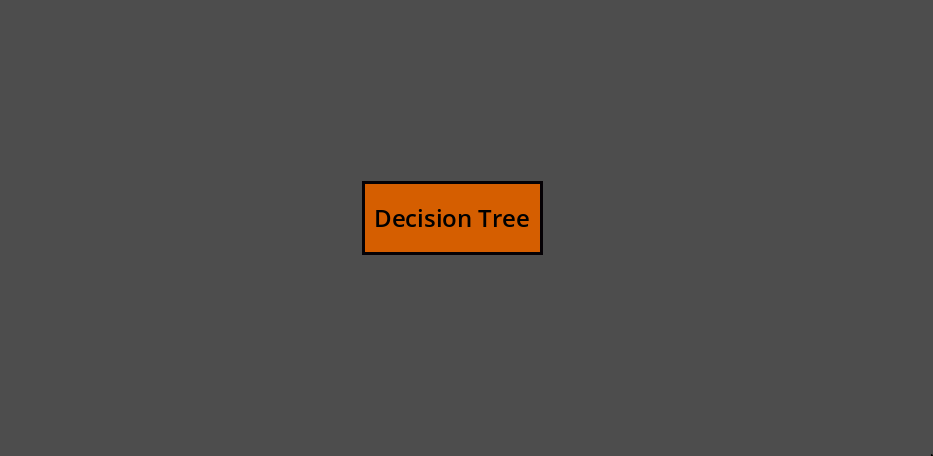
\includegraphics[width=0.75\textwidth]{imaxes/primera_version_del_main_menu.png}
  \caption{Versión preliminar del menú principal.}
  \label{fig:primera_version_del_main_menu}
\end{figure}

Al pulsar el botón se cambiaba de escena a una en la que se encontraba una entidad de una clase personalizada, el ``DNode''.
Esta clase heredaba de la clase botón y tenía tres atributos más: ``id'', ``parent\_id'', y ``sons\_id''.
Los primeros eran enteros, y el segundo un Array de enteros.
Al hacerle clic se desplegaba un menú con una opción: añadir nodo hijo.
Seleccionarla hacía aparecer un nuevo botón debajo del anterior, conectado por una línea.
Esto se podía hacer cuantas veces se quisiera, y hacía que fueran apareciendo nuevos nodos hijo, que se colocaban uno al lado de otro.
Estos siguientes botones tenían una segunda opción en el menú: eliminar nodo.
Esto eliminaba el nodo y sus hijos.

Por debajo el árbol era un diccionario.
Las claves eran enteros, correspondientes a los ids de los DNodes, y los valores eran los propios DNodes.
Estos eran conectados con otros nodos y colocados en pantalla en base a sus atributos de ``parent\_id'' y ``sons\_id''.

Además, en la escena había otros dos botones arriba a la derecha.
En este momento no hacían nada; eran el inicio de lo que acabaría siendo la funcionalidad de cargar y guardar el árbol, retomada durante el desarrollo del árbol de decisión.
En la Figura \ref{fig:primera_version_arbol} se puede ver el estado de esta primera escena interactiva.

\begin{figure}[hp!]
  \centering
  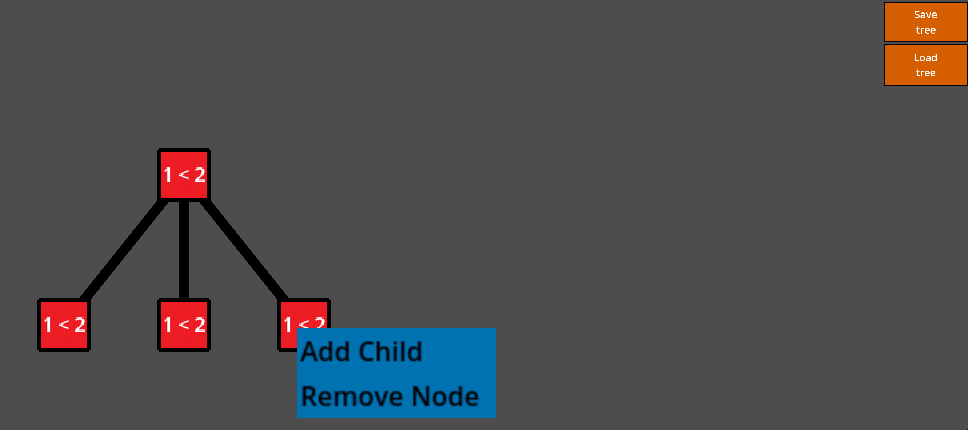
\includegraphics[width=0.75\textwidth]{imaxes/primera_version_arbol.png}
  \caption{Primera escena de prueba para ver el funcionamiento del árbol.}
  \label{fig:primera_version_arbol}
\end{figure}


\subsection{Exportación web con GitHub Pages}

Con esta versión funcional, faltaba probar a exportar a web para comprobar que Godot servía como motor de desarrollo para la aplicación web.
En Godot, para exportar el proyecto a HTML5, hay que descargar las plantillas de exportación, las cuales proporcionan el entorno web base y un archivo HTML que contiene en su estructura el elemento ``<canvas>'', donde el motor (compilado en WebAssembly) inicializa el renderizado gráfico y captura la interactividad.
La prueba se completó sin problemas con un proyecto tan simple.
Más adelante se exploran configuraciones más complejas de la exportación web debido a la creación del plugin para el renderizado de fórmulas.

Después se configuró desde la interfaz web de GitHub la funcionalidad de GitHub Pages.
Para ello, accedí desde la configuración del repositorio a la ventana ``Pages'', desde la cual se puede seleccionar una rama de publicación (para este caso se seleccionó ``main'') y una carpeta para ser la raíz de la página web (en este caso, la carpeta ``docs'', la predeterminada).
Con esta función activada, hubo que exportar el proyecto a la carpeta indicada.
Una vez subidos los cambios a la rama ``main'', la aplicación estaba desplegada.



\section{Árbol de decisión: versión 0.2}

El proyecto dejó de ser un simple mockup cuando se comenzó a trabajar en el primer algoritmo: el árbol de decisión.

\subsection{Primera arquitectura del árbol}

Para comenzar el desarrollo del árbol de decisión, el primer objetivo fue separar la prueba visual inicial de una estructura que pudiera sostener más adelante un algoritmo real. La primera versión del árbol, descrita en la sección anterior, servía para crear nodos manualmente y para comprobar que Godot permitía representar una estructura jerárquica en una escena interactiva. A partir de ese punto se empezó a transformar esa prueba en una vista específica de árbol, con sus propias escenas, scripts y responsabilidades.

La escena principal del proyecto quedó configurada en Godot como un menú simple, implementado como un nodo de tipo ``Control''. Este menú contenía un único botón que al pulsarse llamaba a ``change\_scene\_to\_file'' para cargar la escena del árbol. De esta manera, el menú principal podía crecer en el futuro sin mezclar su lógica con la representación del árbol.

La vista del árbol se organizó dentro de un nodo Control de tipo ``ScrollContainer''.
Este nodo está pensado para tener un solo hijo de tipo Control, y habilita que cuándo este es más grande que la zona que tiene asignada, se pueda scrollear para mover el contenido.
Esta decisión fue importante desde el principio, porque un árbol puede crecer en anchura y altura con rapidez.
Si todos los nodos se colocasen directamente sobre una escena fija, bastarían unos pocos niveles para que parte del árbol quedase fuera de pantalla.
Por ello se creó un ``DTreeCanvas'', el nodo hijo del ScrollContainer, que instanciaba la escena del árbol.
Su función era calcular el tamaño mínimo necesario para contener la estructura completa.
El cálculo partía de los límites del árbol, obtenidos mediante ``get\_tree\_bounds'', y ajustaba ``custom\_minimum\_size'' para que el ScrollContainer pudiera desplazarse hasta todas las zonas relevantes.
%%Dudas: pongo en esta parte que había un nodo de godot que ya me ayudaba con esto, o ya lo digo más adelante?

El núcleo visual del árbol se encapsuló en la clase ``DTreeLogical''.
En su primera versión esta clase heredaba de ``Node2D'' y mantenía un diccionario ``nodes\_dict'', donde cada clave era el identificador de un nodo y cada valor era la instancia visual correspondiente.
También guardaba ``root\_id'', que apuntaba al nodo raíz.
Al iniciarse, el árbol creaba una raíz con identificador 0, la añadía al contenedor de nodos y ejecutaba un reposicionamiento completo.
Esta estructura basada en diccionario permitía acceder a cualquier nodo por su identificador sin recorrer toda la escena de Godot.

El posicionamiento se resolvió mediante un recorrido en orden.
Cada nodo guardaba su profundidad y un índice ``inorder\_index''.
Las hojas recibían índices consecutivos, y los nodos internos se colocaban en el punto medio entre el primer y el último hijo.
Después, ``\_apply\_positions'' multiplicaba esos índices por dos constantes de espaciado, una horizontal y otra vertical.
Con ello se conseguía una distribución simple, estable y suficiente para las primeras pruebas: los hijos aparecían por debajo del padre, y el padre quedaba centrado respecto a ellos.
Tras cada modificación se llamaba a ``relayout\_tree'', que recalculaba índices, posiciones y conexiones.

Las conexiones se implementaron como una escena independiente, ``Conection'', basada en ``Line2D''. En un primer momento la línea solo unía las posiciones globales del nodo padre y del nodo hijo. Más adelante se adaptó para trabajar con nodos de tipo ``Control'', tomando el centro visual de cada botón y convirtiendo esas posiciones al espacio local de la conexión. El contenedor de conexiones recorría ``nodes\_dict'', comprobaba los hijos de cada nodo mediante ``sons\_id'' y creaba una línea por cada relación padre-hijo. Esta separación evitaba que los nodos tuviesen que dibujar sus propias ramas y dejó la responsabilidad de las aristas concentrada en una escena concreta.

El nodo del árbol, ``DNode'', también cambió durante esta primera fase. La versión inicial era un ``Node2D'' con un ``Sprite2D'', un ``Area2D'' y una ``CollisionShape2D''. El ``Area2D'' recibía eventos de ratón, cambiaba el color del sprite al pasar el cursor y abría un menú contextual al hacer clic. Esta solución funcionaba para una prueba gráfica, aunque obligaba a gestionar manualmente colisiones, sprites y etiquetas. En el refactor posterior el nodo pasó a heredar directamente de ``Button''. Con esto se aprovechó el sistema de interfaz de Godot, incluyendo eventos ``gui\_input'', texto incorporado, temas y tamaños de control.

El ``DNode'' conservó las variables necesarias para representar la estructura: ``id'', ``parent\_id'', ``sons\_id'', ``depth'' e ``inorder\_index''. A ellas se añadieron variables relacionadas con el aprendizaje automático, como ``attribute'', ``label'', ``is\_leaf'' y ``branch\_value''. Aunque al principio muchas de ellas todavía no se usaban para ejecutar un algoritmo completo, dejaban preparado el nodo para distinguir entre nodos internos, que representan atributos de división, y nodos hoja, que representan etiquetas de clasificación. También se mantuvo ``can\_remove'', usado para impedir que la raíz pudiese eliminarse desde el modo manual.

La interacción manual quedó coordinada por ``ControllerDTree''. El controlador recibía referencias al árbol, al canvas y a la vista, calculaba el siguiente identificador disponible y conectaba la señal ``change\_child\_requested'' de cada ``DNode''. Cuando un nodo solicitaba añadir un hijo, el controlador instanciaba un nuevo ``DNode'', le asignaba identificador, padre y profundidad, lo añadía a ``nodes\_dict'', lo insertaba en el contenedor visual y registraba su identificador en ``sons\_id'' del padre. Cuando se solicitaba eliminar un nodo, el controlador borraba recursivamente todo su subárbol. Para ello duplicaba la lista de hijos antes de iterar, evitando modificar el array original durante el recorrido, eliminaba el identificador del hijo en el padre, retiraba el nodo del diccionario y liberaba la instancia visual con ``queue\_free''.

En paralelo se crearon dos escenas auxiliares para cargar y guardar árboles. En esta fase eran una funcionalidad preliminar, basada en serializar los atributos estructurales de cada nodo a un archivo JSON en ``user://tree.json''. El guardado recorría ``nodes\_dict'' y extraía identificador, padre, hijos, profundidad e índice de orden. La carga hacía el proceso inverso: leía el JSON, reconstruía instancias de ``DNode'', rellenaba sus atributos y las añadía a un nuevo árbol. Aunque esta persistencia se revisaría bastante más tarde, ya muestra que desde el inicio se pensaba en el árbol como una estructura de datos reconstruible, no solo como elementos colocados manualmente en una escena.

El siguiente cambio relevante fue la preparación del modo automático. El controlador dejó de limitarse a gestionar edición manual y empezó a recibir un modo de funcionamiento, ``manual'' o ``automatic''. En modo manual seguía conectando señales de nodos y permitiendo crear o borrar ramas. En modo automático creaba un panel de control, ``PanelAlgorithmDTree'', con botones para iniciar entrenamiento y avanzar al siguiente paso. Este panel se añadía sobre la vista principal y conectaba sus botones con métodos del controlador. La interfaz todavía era sencilla, con ``Start Training'' y ``Next Step'', y ya introducía el flujo que se mantendría durante el desarrollo: el usuario avanza el algoritmo paso a paso desde la interfaz.

Para ese modo automático se creó la clase ``AlgorithmDTree''. Su primera responsabilidad fue implementar una versión básica de ID3 sobre datos categóricos. El algoritmo guardaba los datos de entrenamiento, la lista de atributos disponibles, una referencia al árbol visual y una pila de llamadas, ``call\_stack'', que permitía convertir una construcción recursiva en una ejecución incremental. Cada contexto de la pila contenía el subconjunto de datos correspondiente, los atributos restantes, el identificador del padre, el valor de la rama por la que se llegaba a ese nodo, la profundidad y un identificador visual todavía pendiente.

El método ``start\_training'' inicializaba el estado y añadía a ``call\_stack'' el contexto de la raíz. A partir de ahí, cada pulsación en ``Next Step'' ejecutaba ``next\_step'', que extraía un contexto de la pila y llamaba a ``\_build\_node\_step''. Esta función concentraba la lógica de decisión. Primero obtenía las etiquetas de los datos. Si todas eran iguales, pedía crear un nodo hoja con esa clase. Si no quedaban atributos, calculaba la clase mayoritaria y creaba una hoja de mayoría. En el resto de casos calculaba la ganancia de información para cada atributo, seleccionaba el atributo con mayor ganancia, preparaba un contexto por cada valor posible del atributo elegido y solicitaba crear un nodo interno.

La entropía se calculó directamente en GDScript. La función ``\_entropy'' contaba ocurrencias de cada etiqueta, transformaba cada conteo en una probabilidad y acumulaba la expresión $-p \log_2(p)$. Sobre esa función se construyó ``\_information\_gain'', que calculaba la entropía total del conjunto, dividía los datos por el valor del atributo y restaba la entropía ponderada de los subconjuntos. Esta implementación fue deliberadamente explícita. En lugar de delegar en una biblioteca externa, el código mostraba de forma transparente los mismos cálculos que después debían explicarse en la interfaz.

La coordinación entre el algoritmo y la escena visual se hizo mediante señales. ``AlgorithmDTree'' emitía ``add\_node\_requested'' indicando padre, valor de rama, atributo, etiqueta y si el nodo era hoja. El controlador recibía esa señal y decidía si debía crear la raíz o un hijo. Para los nodos hijos, actualizaba ``branch\_value'' con el valor del atributo que llevaba hasta ese nodo. Esta variable se usaría poco después para mostrar etiquetas en las conexiones. Como los contextos de los hijos se añadían a la pila antes de saber el identificador real del nodo padre, se introdujo el valor temporal ``-2'' para marcar padres pendientes. Cuando el controlador terminaba de crear un nodo, llamaba a ``update\_pending\_parent\_ids'', que sustituía esos padres pendientes por el identificador recién creado.

Este primer modo automático aún tenía datos de entrenamiento definidos en el propio controlador. El conjunto de prueba contenía frutas descritas mediante atributos categóricos como ``color'', ``shape'' y ``size'', y una columna ``class''. Aunque era un dataset muy pequeño, cumplía dos funciones. Permitía comprobar que la lógica ID3 generaba nodos y ramas, y permitía observar si el árbol visual se actualizaba correctamente en cada paso. A partir de aquí el problema principal dejó de ser crear nodos a mano y pasó a ser sincronizar tres niveles: el estado del algoritmo, la estructura lógica del árbol y la escena que veía el usuario.


\subsection{Reorganización de la vista y primeros elementos explicativos}

Una vez creada la primera versión automática, se reorganizó la escena del árbol para reducir rutas frágiles y separar mejor las responsabilidades. La carpeta inicial ``scenes/views/dtree'' se sustituyó por ``scenes/views/dtree\_view'', y el controlador se movió fuera de la vista, a ``scenes/controllers/controller\_dtree''. Este cambio tenía un objetivo práctico: convertir el controlador en un componente de coordinación capaz de comunicarse con el árbol, la vista, el algoritmo y, más adelante, la ventana informativa.

Durante esta reorganización se probó una estructura con ``SubViewport'' y ``SubViewportContainer'' para poder aplicar zoom al árbol con ``Ctrl'' y la rueda del ratón. La escena contenía un panel inicial con dos opciones, creación manual y creación algorítmica, y el árbol se encontraba dentro de un viewport colocado dentro del ``ScrollContainer''. Esta versión llegó a incluir variables como ``zoom\_level'', ``min\_zoom'', ``max\_zoom'' y ``zoom\_step''. El enfoque añadía complejidad a la entrada de usuario y a los tamaños de la vista. Poco después se retiró esa capa de viewport y el ``DTree'' pasó a ser hijo directo del ``ScrollContainer''. Así se mantuvo el desplazamiento por la vista sin añadir una transformación extra sobre el árbol.

La eliminación del canvas intermedio obligó a revisar el centrado del árbol. En Godot, un ``ScrollContainer'' controla la posición de sus hijos, así que desplazar el propio ``DTree'' no ofrecía un resultado estable. La solución fue mover internamente las posiciones de los nodos. El método ``update\_canvas\_size\_and\_center'' quedó dentro de ``DTreeLogical'', calculando primero el rectángulo de ocupación del árbol, después el tamaño final necesario y, por último, un desplazamiento aplicado a cada nodo. Con este desplazamiento, el contenido del árbol quedaba centrado dentro del área de scroll. Después se actualizaba ``custom\_minimum\_size'' para que las barras del ``ScrollContainer'' conociesen el nuevo tamaño navegable.

También se tuvo en cuenta que el ``ScrollContainer'' actualiza sus barras después de una pasada de layout. Por ese motivo, al centrar el árbol se usó ``set\_deferred'' sobre ``scroll\_horizontal'' y ``scroll\_vertical''. Esta decisión evitaba que Godot limitase el desplazamiento a los valores antiguos justo después de cambiar el tamaño mínimo. Es un detalle pequeño, con un efecto importante para que la vista quedase centrada al crear o modificar el árbol y no apareciese desplazada a una esquina.

La escena ``DTreeView'' empezó a actuar como punto de entrada del flujo de árbol. En ``\_ready'' conectaba los botones del panel de selección, ocultaba el ``ScrollContainer'' y el menú del árbol, y solo mostraba el panel inicial. Al escoger modo manual, hacía visible el árbol, activaba el menú con los botones de carga y guardado, configuraba ``DTreeLogical'' en modo ``manual'' e inicializaba el controlador. Al escoger modo algorítmico, hacía visible el árbol y la ventana, creaba una instancia de ``AlgorithmDTree'', la añadía a la escena y entregaba esa referencia al controlador. Con ello la vista dejó de ser una escena pasiva y pasó a gestionar un flujo de usuario: primero elegir modo, después interactuar con el árbol.

En esta misma fase se creó el autoload ``Constants''. Este script centralizaba identificadores de escenas y temas en dos diccionarios, ``SCENES'' y ``THEMES''. En vez de repetir rutas o UID en scripts distintos, el controlador, el árbol, el menú principal y las conexiones podían acudir a ``Constants.SCENES'' para instanciar escenas como ``dnode'', ``controller\_dtree'', ``panel\_algorithm\_dtree'' o ``conection''. En un proyecto Godot que cambia de carpetas durante el desarrollo, esta centralización reduce errores al mover escenas, porque las referencias se corrigen en un único punto.

La representación visual de los nodos ganó una primera distinción semántica mediante temas. Se añadieron dos recursos ``Theme'': uno para nodos hoja y otro para nodos internos. El tema de hoja usaba una forma más redondeada y un color verdoso, mientras que el tema de nodo interno usaba un color rojizo y esquinas menos redondeadas. ``DNode'' precargaba ambos temas desde ``Constants.THEMES'' y en ``\_ready'' aplicaba uno u otro según ``is\_leaf''. Esta separación hacía que la estructura del árbol se entendiese con menos lectura: los nodos que clasifican y los nodos que dividen los datos tenían una apariencia distinta.

El mismo cambio introdujo ``was\_created\_by\_algorithm''. Los nodos creados por el algoritmo marcaban esta variable a ``true'', y ``DNode'' solo conectaba el menú contextual si el nodo no había sido creado por el modo automático. Esta decisión evitaba que el usuario modificase manualmente nodos que formaban parte de una ejecución algorítmica. El modo manual y el modo automático compartían la misma escena de nodo, aunque su comportamiento frente a clics era distinto. Así se reutilizaba la representación visual sin permitir ediciones que rompiesen la coherencia del entrenamiento paso a paso.

El panel algorítmico también se ajustó a una interfaz más cercana al idioma de la aplicación. Los botones pasaron de ``Start Training'' y ``Next Step'' a ``Empezar entrenamiento'' y ``Siguiente paso''. Además se añadió un botón ``Detalle'', inicialmente poco usado, que anticipaba la necesidad de abrir o actualizar información complementaria. En el controlador se añadieron señales propias, ``next\_step'' y ``detail'', de forma que el botón de siguiente emitía una señal del controlador y esta se conectaba al método ``next\_step'' del algoritmo. Esto desacoplaba la interfaz del algoritmo: el botón ya no llamaba directamente al objeto de entrenamiento.

El nombre del controlador también se corrigió de ``AlgDTree'' a ``ControllerDTree''. Aunque pueda parecer un cambio menor, aclara la responsabilidad de la clase. El algoritmo vive en ``AlgorithmDTree'', mientras que ``ControllerDTree'' se ocupa de conectar botones, señales, nodos visuales, árbol y ventana. Esta separación fue ganando valor en los commits posteriores, porque cada avance del algoritmo requería actualizar la escena, recalcular posiciones, refrescar la ventana o cambiar estados de botones.

Otro cambio de esta etapa fue la creación de una ventana informativa. Primero se añadió directamente como un nodo ``Window'' dentro de ``DTreeView'', con un ``RichTextLabel'' que mostraba el mensaje inicial ``Presiona el botón \"Empezar entrenamiento\"''. Después se extrajo a su propia escena, ``scenes/interface/window/window.tscn'', con su script ``window.gd''. Esta extracción era necesaria para que la ventana tuviese su propia lógica, sus plantillas de texto y su método de actualización, sin llenar ``DTreeView'' de código explicativo.

La ventana comenzó con una posición a la derecha del árbol, cerca de ``(800, 200)'', y después se movió a ``(20, 150)'' con un tamaño de ``300 x 350''. El ajuste mantuvo la lógica y muestra una preocupación temprana por la composición de la escena. La ventana debía estar visible durante el entrenamiento y ocupar un lugar que no estorbase demasiado a la lectura del árbol. En estas primeras versiones seguía siendo una ventana flotante de Godot, bastante distinta de los paneles integrados que se adoptarían más adelante.

El primer contenido de la ventana se construyó con plantillas de texto. ``window.gd'' definía un diccionario ``template\_texts'' con tres casos: ``internal'', ``leaf'' y ``leaf\_mayority''. El texto de nodo interno explicaba cuántos datos habían llegado por la rama, qué etiquetas tenían, qué atributos quedaban, qué métrica se usaba para decidir la división, qué valores obtuvo cada atributo y qué ramas se crearían a partir del mejor atributo. El texto de nodo hoja explicaba el caso en el que todos los datos tenían la misma etiqueta. El texto de hoja por mayoría explicaba el caso en el que ya no quedaban atributos y era necesario escoger la etiqueta más frecuente.

Para alimentar esas plantillas, ``AlgorithmDTree'' empezó a construir un diccionario ``details''. En cada paso se guardaban elementos como ``lista\_etiquetas'', ``numero\_de\_datos'', ``lista\_atributos'', ``tipo\_de\_nodo'', ``mejor\_atributo'', ``valor\_metrica\_mejor\_atributo'', ``lista\_ganancias'' y ``lista\_ramas\_mejor\_atributo''. El controlador llamaba a ``window.update\_current\_text(algorithm.details)'' después de crear cada nodo. De esta forma, la creación visual de un nodo y la explicación asociada quedaban sincronizadas.

La primera versión de esta ventana tuvo problemas porque no todos los campos esperados por las plantillas existían en ``details'', y algunas estructuras se mostraban con formato interno de GDScript. Para corregirlo se completó el diccionario y se añadió un preprocesado en la propia ventana. La función ``\_clean\_lists'' recorría el diccionario y, cuando encontraba arrays de cadenas, los sustituía por una frase con comillas, comas y la conjunción final. Así una lista como ``[\"color\", \"shape\", \"size\"]'' pasaba a mostrarse como ``\"color\", \"shape\", y \"size\"''. Esta transformación era relevante porque la ventana debía ser leída por una persona, no por quien estuviese depurando estructuras de datos.

También se cambió la forma de mostrar las ganancias. Al principio el algoritmo preparaba un diccionario ``ganancias\_info''. La plantilla necesitaba una representación textual, así que se generó ``lista\_ganancias'' concatenando líneas del tipo ``atributo = valor''. La solución todavía era básica, y más tarde se sustituiría por gráficos. En esta fase permitió que la ventana empezase a explicar el criterio de selección de atributo sin depender de la consola de Godot. Esta fue la primera conexión clara entre la matemática del algoritmo y una explicación visible dentro de la aplicación.


\subsection{Animación de la construcción del árbol}

Con la construcción paso a paso funcionando, el siguiente problema fue que la aparición de nodos y ramas resultaba demasiado brusca. Cada pulsación añadía elementos nuevos al árbol, recalculaba posiciones y redibujaba conexiones, de modo que el usuario podía perder el hilo de qué parte acababa de aparecer. Por ello se añadieron animaciones a las ramas y, poco después, a los propios nodos.

La escena ``Conection'' pasó de dibujar una línea completa en cada frame a mantener un progreso de animación, ``\_anim\_progress'', y un estado booleano ``\_animating''. En ``\_ready'' se inicializaba la conexión con progreso cero, se ocultaba la etiqueta poniendo su alfa a cero y se creaba un ``Tween'' que llevaba ``\_anim\_progress'' hasta 1.0 en medio segundo. En paralelo, el mismo ``Tween'' hacía aparecer la etiqueta de la rama. Durante la animación, ``\_process'' llamaba a ``\_update\_from\_progress'', que recalculaba los puntos visibles de la línea.

El cálculo de puntos se concentró en ``\_calc\_points(p)''. Si la conexión no tenía texto, el método interpolaba directamente entre el centro del nodo padre y el centro del nodo hijo. Si tenía texto, la línea se dividía en dos segmentos con un hueco central reservado para la etiqueta. Para ello se calculaba el centro de la conexión, la dirección de la línea, el tamaño mínimo del texto y un margen. Después se obtenían dos puntos de corte alrededor del texto. En vez de dibujar de golpe los dos segmentos, la animación repartía el progreso sobre la longitud total visible. Con esto la rama parecía crecer desde el padre hasta el hijo, respetando el espacio ocupado por la etiqueta.

Esta animación obligó a cambiar el contenedor de conexiones. Antes, cada redibujado eliminaba todas las conexiones y las volvía a crear. Ese enfoque podía servir para una escena estática. Con animaciones provocaba que las ramas existentes volviesen a animarse cada vez que se añadía un nodo nuevo. Para evitarlo, ``ConectionContainer'' empezó a guardar un diccionario ``\_connections'', usando una clave de la forma ``parentId\_childId''. En cada actualización se construía el conjunto de conexiones deseadas a partir de ``sons\_id''. Las conexiones que ya existían se conservaban, las que sobraban se eliminaban y solo se instanciaban las nuevas. Así, al avanzar un paso, se animaba la rama recién creada sin reiniciar el resto del árbol.

Después se añadió una animación de aparición a ``DNode''. Cada nodo comenzaba con ``modulate.a = 0.0'' y un ``Tween'' lo llevaba a opacidad completa en 0.75 segundos con transición sinusoidal. Esto suavizaba tanto la creación de hojas como la creación de nodos internos. La animación era sencilla y cumplía una función didáctica clara: el usuario podía identificar qué elemento era nuevo en el paso actual.

La incorporación de nodos pendientes fue un avance importante. Cuando el algoritmo selecciona un atributo para dividir, ya conoce los valores que darán lugar a ramas, aunque todavía no ha procesado el contenido de cada subrama. Para representar esa situación, la señal ``add\_node\_requested'' se amplió con el parámetro ``children\_branch\_values''. Si el nodo creado era interno, el controlador recibía la lista de valores del atributo y ejecutaba ``\_create\_placeholder\_children''. Este método creaba un ``DNode'' por cada valor de rama, con ``is\_pending = true'', ``text = \"...\"'', ``branch\_value'' asignado y el tema visual de nodo pendiente.

El tema de nodo pendiente se añadió como ``nodedefault'' en ``Constants.THEMES''. Visualmente usaba un color distinto y una forma más redondeada, de modo que se distinguía de las hojas y de los nodos internos definitivos. En términos de interacción, estos placeholders indicaban que el algoritmo ya había decidido que existiría una rama. La decisión concreta de esa rama todavía quedaba pendiente: podía terminar en una hoja o en un nuevo atributo de división. La escena mostraba así un estado intermedio de la construcción, que es más fiel al proceso recursivo que una aparición instantánea de subárboles completos.

Para que los placeholders quedasen asociados a los contextos pendientes del algoritmo, el controlador construía un diccionario ``branch\_to\_id'' con el valor de rama como clave y el identificador del placeholder como valor. Después llamaba a ``algorithm.register\_placeholder\_node\_ids''. El algoritmo recorría su ``call\_stack'' y, para cada contexto cuyo ``parent\_id'' todavía fuese ``-2'', buscaba su ``branch\_value'' en ese diccionario. Si lo encontraba, guardaba el identificador visual en ``node\_id''. De este modo, cuando más adelante se procesaba ese contexto, el controlador podía actualizar el placeholder existente en vez de crear un nodo nuevo.

La actualización de placeholders también se refinó visualmente. En una primera versión, al resolver un placeholder se cambiaban directamente ``attribute'', ``label'', ``text'', ``is\_leaf'', ``is\_pending'' y ``theme''. El cambio era funcional, aunque resultaba abrupto. Para suavizarlo se añadió ``apply\_theme\_animated'' a ``DNode''. Este método hacía desaparecer el nodo, cambiaba el tema y el texto en una llamada de ``tween\_callback'', y volvía a mostrarlo. Así, el paso de ``...'' a un atributo o una etiqueta tenía una transición perceptible.

Otro recurso temprano para explicar el cálculo fue mostrar información al pasar el cursor por un nodo. El algoritmo empezó a enviar un ``info\_value'' junto a la señal de creación de nodo. Para nodos internos, ese valor era la mejor ganancia formateada con dos decimales. ``DNode'' incorporó ``information\_variable\_value'' y conectó ``mouse\_entered'' y ``mouse\_exited''. Al entrar el cursor, el texto del botón se sustituía por ese valor; al salir, volvía a mostrarse el atributo o la etiqueta. Primero se aplicó a la raíz, y después se corrigió la actualización de placeholders para que los nodos hijos también recibiesen esa información.

Esta solución de hover permitía inspeccionar valores numéricos sin llenar todos los nodos con números de forma permanente. El árbol seguía mostrando atributos y clases como texto principal, mientras que la métrica quedaba disponible bajo demanda. Más adelante esta idea se trasladaría hacia la ventana informativa y al clic sobre nodos. En esta fase sirvió para comprobar que cada nodo podía almacenar información explicativa propia.


\subsection{Gráficas y casos explicativos en la ventana}

La ventana informativa evolucionó después de texto plano a una composición con texto, scroll y gráficos. Se creó la escena ``BarsChart'', implementada como un contenedor vertical. El script recibía un título y un diccionario ``data\_to\_plot'' de cadenas a valores reales. En ``\_ready'', por cada clave del diccionario creaba una etiqueta con el nombre del atributo, un ``ColorRect'' cuya anchura dependía del valor multiplicado por ``scale\_mult'', y una etiqueta numérica con el valor formateado a dos decimales. Esta escena permitía comparar visualmente los valores calculados para cada atributo.

Para integrar la gráfica, ``window.tscn'' dejó de usar un único ``RichTextLabel'' y pasó a contener un ``ScrollContainer'' con un ``VBoxContainer''. Dentro de ese contenedor había dos etiquetas, ``Label0'' y ``Label1'', y una instancia de ``BarsChart''. Las plantillas de texto pasaron de ser cadenas únicas a arrays de fragmentos. En el caso de un nodo interno, la primera parte explicaba los datos y atributos disponibles, después se insertaba la gráfica y la segunda parte explicaba qué atributo había sido escogido y qué ramas se crearían. Esta estructura hacía que el gráfico quedase integrado en la explicación.

El método ``update\_current\_text'' de la ventana empezó a tratar ``lista\_ganancias'' como un diccionario cuando era posible. Antes de añadir un gráfico nuevo, buscaba si ya existía un nodo ``BarsChart'' en el contenedor y lo eliminaba. Después añadía una nueva instancia creada con ``BarsChart.newone(\"Entropía por atributo\", plot\_data)'' y recolocaba ``Label1'' al final. Esta limpieza evitaba que la ventana acumulase gráficos de pasos anteriores.

Al mismo tiempo, la ventana ganó su propia lógica de scroll. Igual que en la vista principal, se añadieron variables para arrastre con botón central y rueda del ratón. Esto era útil porque la explicación empezaba a ocupar más altura que la ventana. La interfaz de detalle dejaba de ser un texto corto fijo y empezaba a comportarse como un panel de lectura, con contenido variable según el tipo de nodo y según el número de atributos.

El algoritmo también se adaptó a esta representación. ``details[\"lista\_ganancias\"]'' pasó a guardar directamente un ``Dictionary[String, float]''. Con ello ``BarsChart'' podía usar los valores numéricos reales, sin tener que interpretar una cadena previamente formateada. La función ``\_information\_gains\_for\_all\_atributes'' se tipó como un diccionario de cadenas a reales, reforzando la idea de que esos valores eran datos para la interfaz, no solo texto para imprimir.

Se añadió un caso específico para empates entre atributos. Tras calcular las ganancias, el algoritmo recorría el diccionario y contaba cuántos atributos tenían el valor máximo. Si solo había uno, ``details[\"tipo\_de\_nodo\"]'' seguía siendo ``internal''. Si había varios, pasaba a ser ``internal\_multi\_atribute'' y se guardaba ``n\_atributos\_con\_ganancia\_maxima''. La ventana incorporó una plantilla para este caso, explicando que varios atributos compartían la mejor métrica y que se continuaba con uno de ellos. Esta explicación era necesaria para que la elección no pareciese arbitraria cuando los datos daban varias divisiones equivalentes.

La redacción de los nodos hoja también se ajustó al probar datasets más grandes. La plantilla inicial decía que solo había bajado un dato por la rama, algo que era cierto en el primer dataset de frutas. La frase dejaba de encajar en cuanto varios ejemplos con la misma clase llegaban a la misma hoja. El texto pasó a decir que habían bajado ``{numero\_de\_datos}'' datos con la misma etiqueta. Este cambio muestra cómo la explicación dependía de probar casos distintos: al ampliar los datos, aparecían frases demasiado específicas que había que generalizar.


\subsection{Primer panel de selección de datasets}

Hasta ese momento, los datos de entrenamiento estaban incrustados en el controlador. Esto facilitaba las primeras pruebas y limitaba la aplicación a un único ejemplo. El siguiente paso fue separar la selección de datos del arranque del entrenamiento. Primero se probó un segundo dataset definido también en código, con atributos ``tipo'', ``estado'' y ``tamaño'', y una etiqueta ``clase''. Este conjunto incluía rocas, animales y plantas, con casos puros, casos mezclados y contradicciones diseñadas para forzar ramas más profundas. El objetivo era comprobar que el árbol se comportaba bien cuando la columna objetivo no se llamaba ``class''.

Para conseguirlo se añadió ``label\_column'' a ``AlgorithmDTree''. La función ``\_get\_labels'' dejó de acceder siempre a ``row[\"class\"]'' y pasó a leer ``row[label\_column]''. El controlador infería esa columna buscando en las claves del primer dato aquella que no estuviese en la lista de atributos. Esta solución todavía era simple y hacía posible entrenar con datasets que usasen nombres de etiqueta distintos, como ``clase''. Con ello el algoritmo quedaba menos acoplado al primer ejemplo de frutas.

Después se creó ``PanelDatasetSelection''. La escena era un ``PanelContainer'' con un título, dos botones grandes para ``Frutas'' y ``Csv'', un panel de texto informativo y un botón ``Entrenar''. Al principio el script solo guardaba la opción seleccionada y dejaba la carga de CSV como una función vacía. En la siguiente iteración se completó la lógica: el panel contenía ``DICT\_OF\_DATASETS'' con el dataset de frutas y sus atributos, deshabilitaba el botón de entrenamiento hasta que hubiese una selección válida, mostraba mensajes de éxito o error en colores distintos y emitía ``SignalsObserver.dataset\_selected'' con los datos y atributos.

La opción de CSV introdujo una primera carga desde archivo. Al pulsar ``Csv'', el panel creaba un ``FileDialog'', lo configuraba para seleccionar archivos ``*.csv'', intentaba usar el selector nativo si estaba disponible y conectaba ``file\_selected'' con ``\_parse\_csv''. La función de parseo abría el archivo, leía la primera fila como cabeceras, recorría las filas restantes con ``get\_csv\_line'' y construía un diccionario por fila, asignando cada cabecera a su valor. Si el archivo se abría correctamente, el panel guardaba el array de diccionarios, tomaba las cabeceras como atributos y habilitaba el entrenamiento.

Para mantener tipos explícitos en el resto del código, el panel añadió ``safe\_get\_array\_of\_dicts'' y ``safe\_get\_array\_of\_strings''. Estas funciones convertían arrays genéricos en ``Array[Dictionary]'' y ``Array[String]'' comprobando elemento a elemento. La razón estaba en una limitación práctica de Godot con tipos anidados complejos: el diccionario de datasets predefinidos mezclaba arrays de datos y arrays de atributos, y después era necesario entregar valores con tipos más concretos al controlador y al algoritmo.

La integración con la vista cambió el flujo del modo algorítmico. Al pulsar ``Algoritmicamente'', ``DTreeView'' ocultaba el panel de selección de modo y mostraba ``PanelDatasetSelection''. El controlador, por su parte, conectaba ``SignalsObserver.dataset\_selected'' con ``\_on\_start\_training\_pressed''. Cuando el usuario pulsaba ``Entrenar'', el panel emitía los datos, se ocultaba, y el controlador guardaba ``data'' y ``attributes'', configuraba ``label\_column'', llamaba a ``algorithm.start\_training'' y hacía visible el botón ``Siguiente paso''. Esta separación convirtió el entrenamiento en un flujo más claro: primero se elige un dataset, después se construye el árbol.

Esta versión del panel todavía tenía partes provisionales. La visibilidad del árbol y de la ventana tras seleccionar dataset se terminaría de ajustar en el siguiente bloque de trabajo, y la carga de CSV todavía trataba todas las cabeceras como atributos, por lo que era necesario mejorar la detección de la columna objetivo. Aun así, el cambio fue relevante porque eliminó el botón ``Empezar entrenamiento'' del panel algorítmico y trasladó el arranque real del algoritmo a una selección explícita de datos.


\subsection{Carga de CSV y navegación por pasos}

El primer ajuste tras introducir el panel de datasets fue hacer que la carga de CSV fuese usable para entrenar. Se añadió una lista de nombres habituales para la columna objetivo, ``class'', ``Class'', ``y'', ``Y'', ``label'' y ``Label''. Al leer un CSV, el panel convertía las cabeceras a ``Array[String]'' con ``safe\_get\_array\_of\_strings'' y, una vez cargadas las filas, eliminaba de la lista de atributos la primera cabecera que coincidiese con uno de esos nombres. Así el array ``attrs\_info'' dejaba de incluir la etiqueta, y el controlador podía detectar la columna objetivo como la diferencia entre las claves del dato y los atributos.

También se corrigió la lectura de filas. En Godot, ``eof\_reached'' se activa después de intentar leer más allá del final, por lo que el bucle inicial podía resultar incómodo de razonar. La versión corregida usaba un ``while true'', leía una fila con ``get\_csv\_line'', comprobaba después si se había alcanzado el final y salía del bucle en ese caso. Las filas vacías se ignoraban y cada fila válida se convertía en un diccionario. Este parseo seguía siendo sencillo y ya era suficiente para cargar datasets categóricos externos con una cabecera y varias filas.

La vista del árbol ajustó su visibilidad al nuevo flujo. Al escoger el modo algorítmico se mostraba el panel de selección de dataset, mientras que el árbol y la ventana quedaban ocultos. Después de recibir ``SignalsObserver.dataset\_selected'', se mostraban el ``ScrollContainer'' y la ventana. Con ello el usuario no veía un árbol vacío ni una ventana de explicación antes de haber elegido los datos. El texto inicial de la ventana se cambió a ``Presiona el botón \"Siguiente\"'', porque el entrenamiento ya empezaba al seleccionar el dataset y no al pulsar un botón de entrenamiento dentro del panel algorítmico.

En ese mismo momento empezó a prepararse la navegación hacia atrás. Se añadió la señal ``previous\_step'' al controlador, se conectó con el algoritmo y se creó un método ``previous\_step'' en ``AlgorithmDTree''. La primera versión solo movía el último contexto de ``called\_stack'' de vuelta a ``call\_stack'' y llamaba a ``\_unbuild\_node\_step'', que todavía estaba vacío. Aunque no deshacía nada, este cambio ya introducía las estructuras necesarias: una pila de pasos pendientes, ``call\_stack'', y otra de pasos ejecutados, ``called\_stack''.

Después se añadió el botón ``Paso previo'' al panel del algoritmo. La escena ``panel\_algorithm\_dtree.tscn'' incorporó ``PrevButton'', y el controlador guardó una referencia ``previous\_step\_button'', conectó su pulsación con ``\_on\_previous\_step\_button\_pressed'' y lo hizo visible al comenzar el entrenamiento. Desde la interfaz, el modo de construcción del árbol dejaba de ser estrictamente lineal. El usuario podía avanzar con ``Siguiente paso'' y retroceder con ``Paso previo'', una característica importante para una herramienta didáctica, porque permite revisar el punto exacto en el que aparece una rama o se decide una hoja.

La implementación real del retroceso se hizo en ``\_unbuild\_node\_step''. El algoritmo comprobaba primero que existiese una referencia válida al árbol y resolvía qué nodo visual correspondía al contexto que se quería deshacer. Para ello se añadió ``\_resolve\_context\_node\_id''. Este método intentaba usar ``context[\"node\_id\"]'' si ya estaba disponible. Si no lo estaba, buscaba el nodo raíz cuando el padre era ``-1'', o recorría los hijos del padre comparando ``branch\_value''. Esta segunda vía era necesaria porque algunos contextos se asociaban a placeholders creados antes de que el nodo se resolviese por completo.

Antes de borrar un nodo, el algoritmo determinaba si el contexto correspondía a un nodo interno con ``\_is\_internal\_context''. Para ello reutilizaba las mismas condiciones de construcción: si todas las etiquetas eran iguales, el contexto era una hoja; si no quedaban atributos, también era una hoja; en otro caso se trataba como un nodo interno. Cuando se deshacía un nodo interno, primero se eliminaban de ``call\_stack'' los contextos de sus hijos mediante ``\_remove\_child\_contexts\_for\_parent'', y después se eliminaban visualmente sus hijos con ``\_remove\_visual\_children\_for\_node''. Así se evitaba dejar en la pila tareas que dependían de un nodo que acababa de desaparecer.

La forma de deshacer dependía del origen del nodo. Si el contexto correspondía a la raíz, se eliminaba todo el subárbol y se ponía ``root\_id'' a ``null''. Si el nodo procedía de un placeholder, se restauraba como pendiente en lugar de borrarlo. Esto se hizo con ``restore\_node\_as\_pending'', que limpiaba ``attribute'', ``label'' e ``information\_variable\_value'', ponía ``is\_leaf'' a ``false'', ``is\_pending'' a ``true'' y llamaba a ``apply\_theme\_animated'' con el tema de pendiente y el texto ``...''. Si el nodo no procedía de un placeholder, se eliminaba con ``remove\_subtree\_and\_self''.

Para soportar ese borrado, ``DTreeLogical'' incorporó ``remove\_subtree\_and\_self''. El método comprobaba que el nodo existiese, duplicaba su lista de hijos, eliminaba cada subárbol de forma recursiva, retiraba el identificador del nodo en el padre, borraba la entrada de ``nodes\_dict'', actualizaba ``root\_id'' si era necesario y liberaba la instancia visual. Esta función era parecida al borrado del modo manual y quedó dentro del propio árbol para que el algoritmo pudiera usarla al deshacer pasos.

Al probar el retroceso apareció un problema al volver al paso cero: si el árbol quedaba vacío, el reposicionamiento no redibujaba las conexiones. La corrección consistió en hacer que ``relayout\_tree'' comprobaba si ``root\_id'' era ``null'' o si ``nodes\_dict'' estaba vacío. En ese caso llamaba igualmente a ``\_redraw\_edges'' y terminaba. Así el contenedor de conexiones podía eliminar las ramas que ya no existían. El controlador también reactivaba el botón de siguiente al pulsar ``Paso previo'', porque deshacer un paso debe permitir avanzar de nuevo.


\subsection{Primera evaluación visual del árbol}

El último avance de este tramo inicial fue una primera versión del modo de evaluación. Hasta entonces, la aplicación había mostrado cómo se construía el árbol; el uso de ese árbol para clasificar datos nuevos quedaba pendiente. La evaluación se introdujo con un enfoque visual: un dato de prueba se representaría como un objeto que cae por el árbol siguiendo las ramas marcadas por sus atributos.

El panel algorítmico incorporó dos botones nuevos: ``Evaluar'' y ``Dropear dato''. Durante el entrenamiento, ``Evaluar'' permanecía deshabilitado. Cuando el algoritmo emitía ``algorithm\_completed'', el controlador deshabilitaba ``Siguiente paso'' y habilitaba ``Evaluar''. Al pulsarlo, se ocultaban los botones de construcción y se volvía a mostrar el panel de selección de dataset. Esta reutilización del panel permitía escoger datos para probar el árbol después de haberlo entrenado.

El controlador empezó a distinguir entre dos fases mediante ``has\_train\_started''. La primera vez que recibía ``dataset\_selected'', guardaba los datos, configuraba el algoritmo e iniciaba el entrenamiento. Las siguientes veces interpretaba la selección como datos de evaluación, hacía visible ``Dropear dato'' y emitía ``SignalsObserver.start\_evaluation''. Esta solución era provisional y permitía reutilizar la misma señal global para entrenamiento y evaluación sin crear todavía una interfaz separada para cada fase.

Para representar cada muestra se creó ``EvalData''. Era una escena pequeña basada en ``Node2D'', con un ``ColorRect'' como forma visual y una variable ``data\_dict'' donde se guardaba el diccionario de atributos de la muestra. La función estática ``newone'' instanciaba la escena, asignaba el diccionario y devolvía el objeto listo para colocarse en la vista.

La lógica del recorrido quedó en ``EvalDataContainer''. Esta escena recibía el árbol entrenado y una lista de ``EvalData''. Al crearse, copiaba la información relevante de cada nodo del árbol a un diccionario ``nodes'': posición, profundidad, atributo, etiqueta, valor de rama y padre. Esta copia era útil porque el dato evaluado necesitaba recorrer la estructura aunque el algoritmo original ya hubiese terminado. El contenedor se conectaba a ``SignalsObserver.drop\_data'', de modo que cada pulsación en ``Dropear dato'' ejecutaba ``\_drop\_one\_data''.

El método ``\_drop\_one\_data'' tomaba la primera muestra pendiente, la añadía como hija del contenedor y buscaba la raíz identificando el nodo con profundidad cero. Después entraba en un bucle. En cada iteración movía el objeto ``EvalData'' hasta la posición del nodo actual con un ``Tween'' de 0.35 segundos y esperaba a que terminase. Si el nodo actual tenía etiqueta, el recorrido terminaba, porque se había llegado a una hoja. Si era un nodo interno, obtenía el atributo de división, buscaba en ``data\_dict'' el valor de ese atributo y localizaba entre los nodos copiados un hijo cuyo ``parent\_id'' coincidiese con el nodo actual y cuyo ``branch'' coincidiese con el valor de la muestra. Ese hijo pasaba a ser el siguiente nodo.

El algoritmo se conectó a esta fase mediante ``SignalsObserver.start\_evaluation''. En ``\_evaluate\_dtree'', convertía cada diccionario del dataset de evaluación en un ``EvalData'' y añadía a la escena actual un ``EvalDataContainer'' creado con el árbol y la lista de muestras. Las señales globales se ampliaron con ``start\_evaluation'', ``drop\_data'' y ``all\_data\_droped''. La última se emitía cuando ya no quedaban muestras por soltar.

Esta primera evaluación era todavía básica. Los datos se dibujaban como rectángulos simples, el contenedor se añadía directamente a la escena actual y el recorrido completo de una muestra se hacía de una vez hasta la hoja. Las mejoras posteriores, como el movimiento nivel a nivel, el apilado bajo hojas, el color por clase y la explicación de cada decisión en la ventana, pertenecen a una etapa posterior del desarrollo. Aun así, este commit dejó establecida la idea central del modo de evaluación: ver físicamente cómo una muestra atraviesa las decisiones del árbol hasta llegar a una clasificación.

Con este conjunto de cambios quedó completada la primera versión significativa del árbol de decisión. El proyecto pasó de dibujar nodos conectados a construir un árbol ID3 paso a paso, mostrar estados pendientes, animar la aparición de ramas y nodos, explicar la selección de atributos con texto y gráficos, cargar datasets sencillos y ejecutar una primera evaluación visual. A partir de aquí el desarrollo del árbol continuó con mejoras de interfaz, persistencia, adaptación a móvil y explicaciones más completas, que se tratarán en apartados posteriores para no mezclar esta primera fase con las revisiones finales.

 \chapter{Conclusiones}
\label{chap:conclusiones}

El desarrollo realizado permite concluir que los objetivos planteados al inicio del trabajo se han cumplido.
El resultado final es una aplicación educativa interactiva, accesible desde la web, que permite estudiar de forma visual el entrenamiento y la inferencia de un árbol de decisión y de una red neuronal multicapa.
Para llegar a ese resultado se partió del estudio conceptual de ambos algoritmos y se trasladaron sus operaciones fundamentales a una implementación propia en Godot, manteniendo una correspondencia directa entre el cálculo interno, la representación gráfica y las explicaciones mostradas al usuario.

El proceso seguido comenzó con la validación de Godot como entorno adecuado para construir una aplicación interactiva exportable a navegador.
Esta primera fase permitió comprobar que era posible representar estructuras dinámicas, modificar elementos durante la ejecución y desplegar el proyecto mediante GitHub Pages.
A partir de esa base se incorporó el árbol de decisión, pasando de una estructura editable manualmente a una construcción guiada por el algoritmo ID3.
La aplicación permite observar cómo se crean los nodos, cómo se seleccionan los atributos mediante la métrica basada en entropía y cómo se forman las hojas.
La ventana informativa, las gráficas y la navegación por pasos convierten ese proceso en una explicación progresiva, en la que cada decisión del algoritmo queda asociada a los datos que la provocan.

El segundo bloque principal fue la red neuronal.
Su desarrollo exigió representar una arquitectura formada por capas, neuronas y conexiones densas, y vincular esa representación con un modelo lógico que conserva pesos, sesgos, funciones de activación y parámetros de entrenamiento.
La aplicación permite configurar la red según el conjunto de datos, ejecutar el forward pass paso a paso, mostrar el cálculo de cada neurona, comparar la salida con el valor esperado y representar el backward pass mediante la actualización visible de los parámetros.
De esta forma, el entrenamiento deja de presentarse como una operación opaca y pasa a mostrarse como una secuencia de predicciones, errores y correcciones sobre el modelo.

La fase final del desarrollo consolidó la aplicación como recurso educativo.
Se revisó la navegación general, se adaptaron las vistas a distintos tamaños de pantalla, se mejoró la legibilidad visual de los algoritmos, se integró el renderizado de fórmulas matemáticas y se reforzaron las validaciones de datos.
También se completaron los modos de evaluación tanto en el árbol, donde los datos recorren las ramas aprendidas hasta llegar a una hoja, como en la red, donde la inferencia reutiliza el forward pass sin modificar los parámetros entrenados.
Estas funciones permiten observar no solo cómo se obtiene un modelo, sino también cómo se utiliza después para clasificar o predecir nuevos ejemplos.

El trabajo ha permitido adquirir competencias directamente relacionadas con los objetivos propuestos.
La implementación desde cero de los algoritmos obligó a comprender sus parámetros, sus estructuras internas y las condiciones que aparecen durante su ejecución.
La construcción de la interfaz exigió organizar Escenas, Señales, paneles, animaciones y elementos informativos para que la interacción fuera comprensible.
El despliegue web, junto con la carga y descarga de archivos en navegador, amplió el alcance técnico del proyecto y permitió que la aplicación pudiera consultarse como recurso público de aprendizaje.

En conjunto, el proyecto cumple el propósito principal de ofrecer una herramienta que ayude a comprender paso a paso el funcionamiento interno de dos modelos básicos de aprendizaje automático.
La aplicación final no se limita a mostrar el resultado de un entrenamiento, sino que hace visible el proceso que conduce a ese resultado, acompaña los cálculos con texto, fórmulas y gráficas, y permite experimentar con datos y configuraciones desde una interfaz accesible en web.

 \chapter{Trabajo futuro}
\label{chap:trabajo_futuro}

El desarrollo realizado deja una base sobre la que pueden plantearse varias ampliaciones. La aplicación actual se centra en dos modelos concretos, árboles de decisión y redes neuronales multicapa, y los presenta de forma incremental para que el usuario pueda seguir tanto el entrenamiento como la evaluación. A partir de esa base, el trabajo futuro puede organizarse en tres líneas principales: ampliar el catálogo de algoritmos, profundizar en las opciones de los modelos ya implementados e integrar el aprendizaje con simulaciones interactivas creadas en el propio motor.

\section{Ampliación del catálogo de modelos}

Una primera línea de evolución consiste en incorporar nuevos algoritmos de aprendizaje automático. La estructura modular desarrollada para separar algoritmo, representación visual y ventana informativa facilita que la aplicación pueda crecer con nuevos modelos, siempre que cada uno se acompañe de una visualización adaptada a su forma de aprender.

En el caso de las redes neuronales, una extensión natural sería incluir topologías más variadas. La versión actual trabaja con redes densas multicapa, suficientes para explicar el forward pass, el cálculo del error y la retropropagación. A partir de ahí, podrían añadirse arquitecturas convolucionales, recurrentes o basadas en mecanismos de atención. Cada una de ellas permitiría trabajar conceptos nuevos: filtros y mapas de características en redes convolucionales, dependencias temporales en redes recurrentes o matrices de atención en modelos de tipo transformer.

Los transformadores tendrían un interés especial como línea futura por su presencia en muchos sistemas actuales de aprendizaje automático. Su incorporación requeriría representar elementos distintos a los de una red densa clásica, como tokens, embeddings, cabezas de atención y bloques sucesivos de procesamiento. Esta ampliación exigiría una visualización más compleja, con relaciones simultáneas entre muchos elementos y conexiones que van más allá de las capas consecutivas de una red densa.

La incorporación de nuevos modelos también permitiría comparar enfoques. La aplicación podría mostrar cómo distintos algoritmos resuelven un mismo conjunto de datos, qué información utiliza cada uno y qué tipo de explicación resulta más adecuada en cada caso. Esta comparación reforzaría el objetivo didáctico del proyecto, ya que ayudaría a entender que el aprendizaje automático agrupa técnicas con estructuras y procesos de decisión muy diferentes.

\section{Profundización en los modelos existentes}

Una segunda línea de trabajo consiste en enriquecer los algoritmos que ya forman parte de la aplicación. En el árbol de decisión, una mejora directa sería permitir distintos criterios de división. La versión actual se apoya en una métrica basada en entropía e información, por lo que el usuario sigue siempre el mismo tipo de razonamiento al crear cada nodo. Incluir alternativas como el índice Gini o el ratio de ganancia permitiría comparar cómo cambia la elección de atributos según la medida utilizada.

También sería relevante ampliar el tipo de datos aceptados por el árbol. En su estado actual, el algoritmo trabaja con atributos categóricos. Para manejar atributos numéricos continuos habría que buscar umbrales de corte y explicar por qué un valor separa mejor los datos que otros posibles valores. Esta mejora enriquecería la visualización, ya que la ventana informativa podría mostrar la comparación entre atributos y, dentro de cada atributo numérico, la comparación entre posibles puntos de división.

Otra ampliación posible para el árbol sería incorporar técnicas de poda o mecanismos de control de crecimiento. Con ello, el usuario podría observar la diferencia entre construir un árbol que se ajusta mucho a los datos de entrenamiento y construir una estructura más sencilla con mejor capacidad de generalización. Esta línea conectaría la visualización del algoritmo con problemas habituales del aprendizaje automático, como el sobreajuste y la validación del modelo.

En la red neuronal, el trabajo futuro puede avanzar hacia una configuración más flexible del entrenamiento. Algunas opciones posibles son permitir distintos optimizadores, modificar la tasa de aprendizaje durante la ejecución, elegir funciones de pérdida alternativas o incorporar regularización. Cada una de estas decisiones afecta al modo en el que cambian los pesos, por lo que la aplicación podría mostrar sus efectos de forma visual durante el backward pass.

La red también podría dejar de limitarse a conexiones densas. Permitir topologías no densas o definidas por el usuario abriría la puerta a explicar cómo cambia el flujo de información cuando una neurona no está conectada con todas las neuronas de la capa siguiente. Esta mejora mantendría la relación entre arquitectura visible y modelo lógico, a la vez que daría más importancia a la estructura de conexiones como parte del aprendizaje.

Todas estas ampliaciones comparten una misma condición: las nuevas opciones deberían integrarse sin perder el carácter explicativo de la herramienta. Añadir parámetros o variantes del algoritmo tendría sentido si la aplicación muestra qué cambia en el cálculo, qué decisión se toma y qué consecuencia tiene sobre el modelo final.

\section{Integración con simulaciones interactivas}

La tercera línea de trabajo es la más vinculada con la elección de Godot como herramienta de desarrollo. Una evolución especialmente interesante sería conectar los algoritmos con una simulación o un videojuego ejecutándose en la propia aplicación. En ese escenario, el entorno interactivo generaría datos durante la ejecución, y el modelo aprendería a partir de lo que sucede en la escena.

Esta integración permitiría pasar de datasets estáticos a datos producidos por una dinámica viva. Por ejemplo, una escena podría generar posiciones, acciones, colisiones, decisiones de un personaje o resultados obtenidos tras cada intento. Esos eventos podrían convertirse en entradas para un modelo, y la respuesta del modelo podría influir de nuevo en el comportamiento de la simulación. El usuario observaría entonces dos procesos conectados: la evolución del entorno y la evolución del algoritmo que aprende a partir de él.

Una línea de este tipo serviría también para explorar problemas cercanos al aprendizaje por refuerzo. Un agente podría recibir información del estado del juego, escoger acciones y obtener recompensas según lo ocurrido. La visualización tendría que mostrar tanto la ejecución del agente como la actualización interna del modelo. Esto ampliaría el proyecto hacia una dimensión más experimental, donde la explicación del aprendizaje estaría ligada a consecuencias visibles dentro de una escena interactiva.

Esta posibilidad refuerza la justificación del uso de Godot. El motor actuaría como soporte para dibujar interfaces, entorno de simulación, generador de datos y medio de interacción. Además, la exportación a HTML5 permitiría mantener el acceso desde navegador incluso en versiones más cercanas a una experiencia de juego educativo.

En conjunto, estas tres líneas de trabajo permitirían hacer crecer la aplicación en amplitud, profundidad y conexión con entornos interactivos. La prioridad debería seguir siendo la misma que en la versión actual: que cada avance del algoritmo pueda observarse, que cada decisión esté acompañada por una explicación y que la visualización ayude a entender el funcionamiento interno del modelo.


 %%%%%%%%%%%%%%%%%%%%%%%%%%%%%%%%%%%%%%%%
 % Apéndices, glosarios e bibliografía  %
 %%%%%%%%%%%%%%%%%%%%%%%%%%%%%%%%%%%%%%%%

%\appendix
%\appendixpage
%\chapter{Material adicional}
\label{chap:adicional}

\lettrine{E}{n} este apéndice se muestran más imágenes del proceso de desarrollo del proyecto.


\begin{figure}[H]
  \centering
  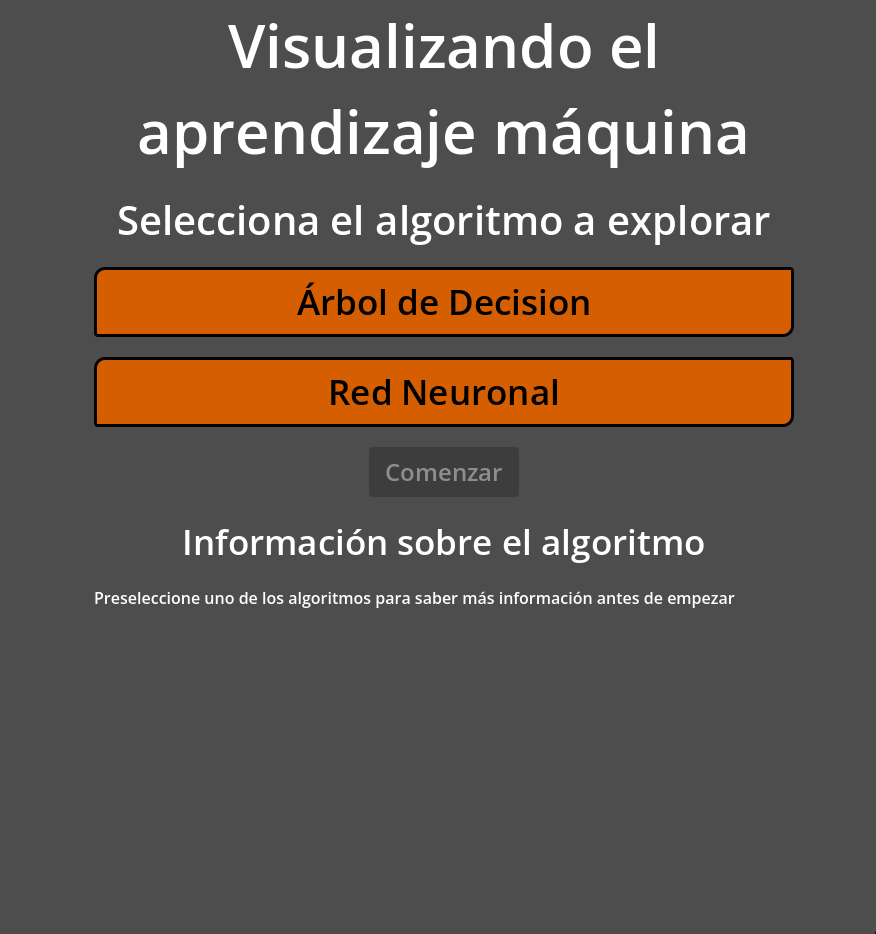
\includegraphics[width=0.7\textwidth]{imaxes/a_mm_2.png}
  \caption{Una de las iteraciones del menú principal.}
  %\label{fig:}
\end{figure}

\begin{figure}[H]
  \centering
  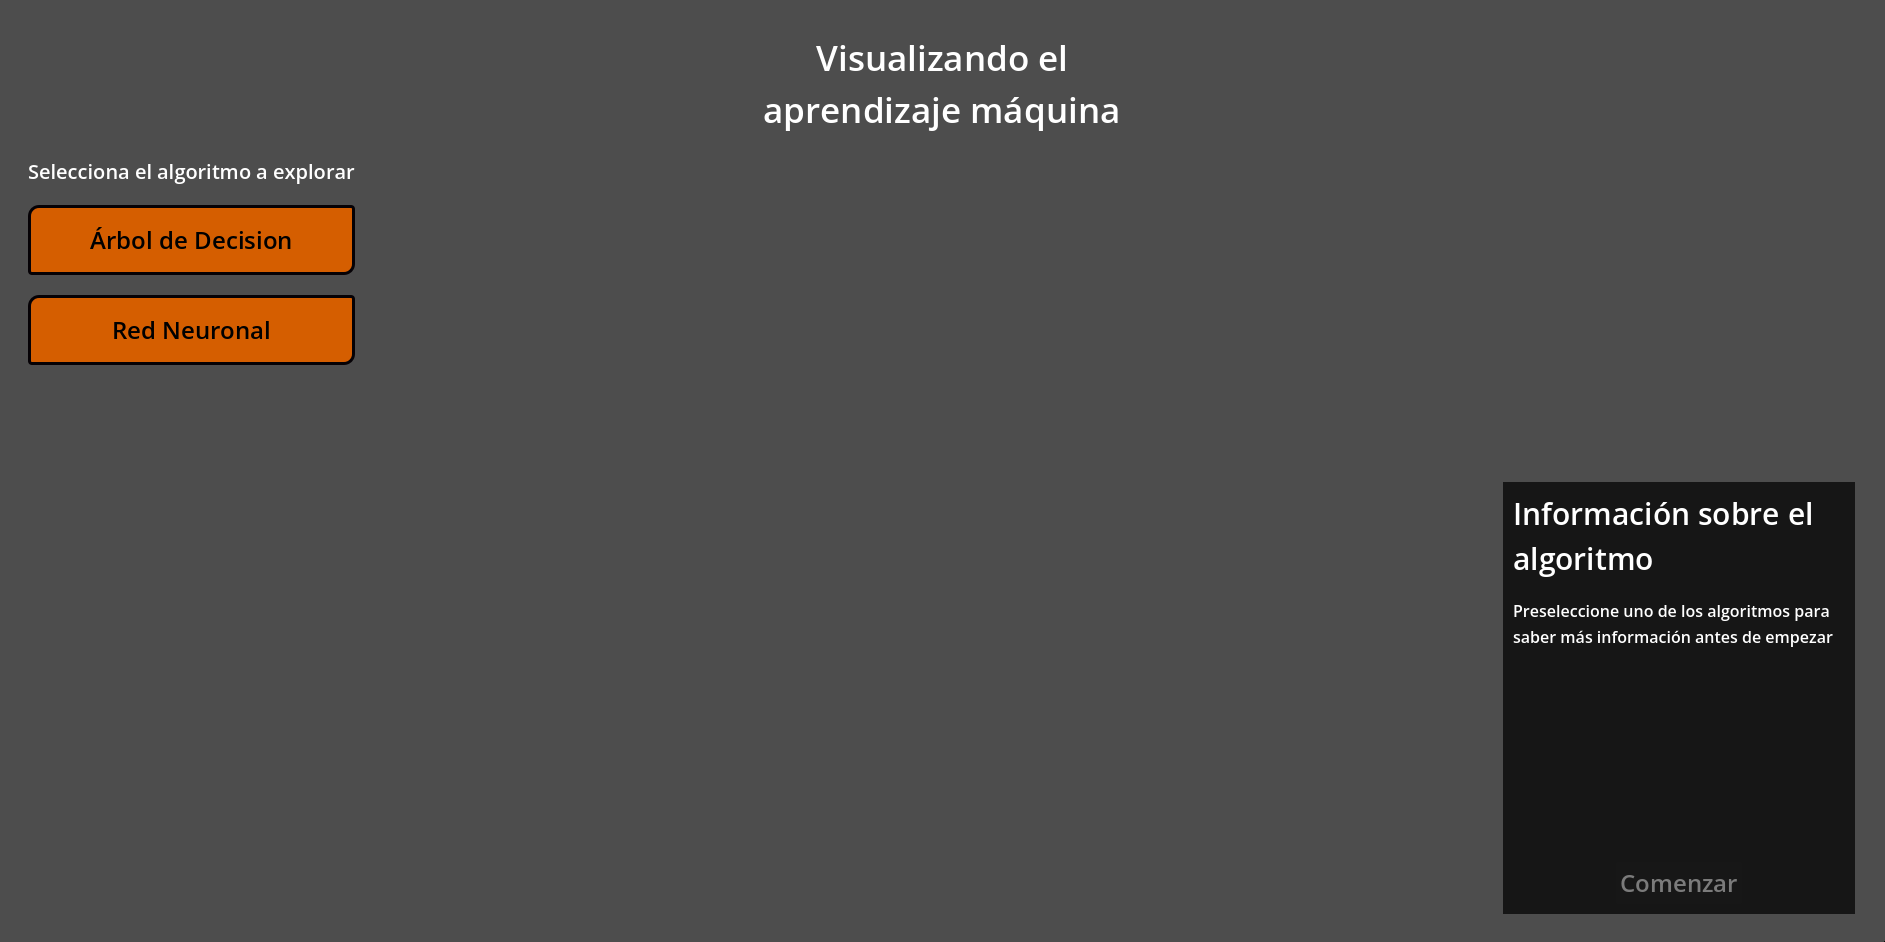
\includegraphics[width=0.7\textwidth]{imaxes/a_mm_1.png}
  \caption{Una de las iteraciones del menú principal.}
  %\label{fig:}
\end{figure}

\begin{figure}[H]
  \centering
  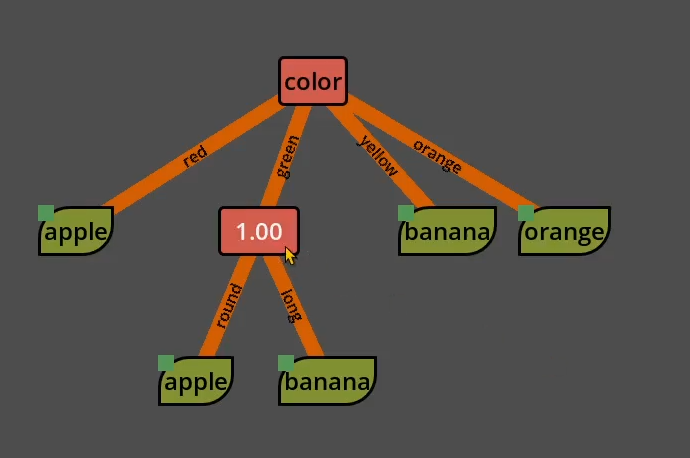
\includegraphics[width=0.7\textwidth]{imaxes/a_numeromal.png}
  \caption{Forma en la que se mostraba la pureza de un nodo en la primera versión.}
  %\label{fig:}
\end{figure}

\begin{figure}[H]
  \centering
  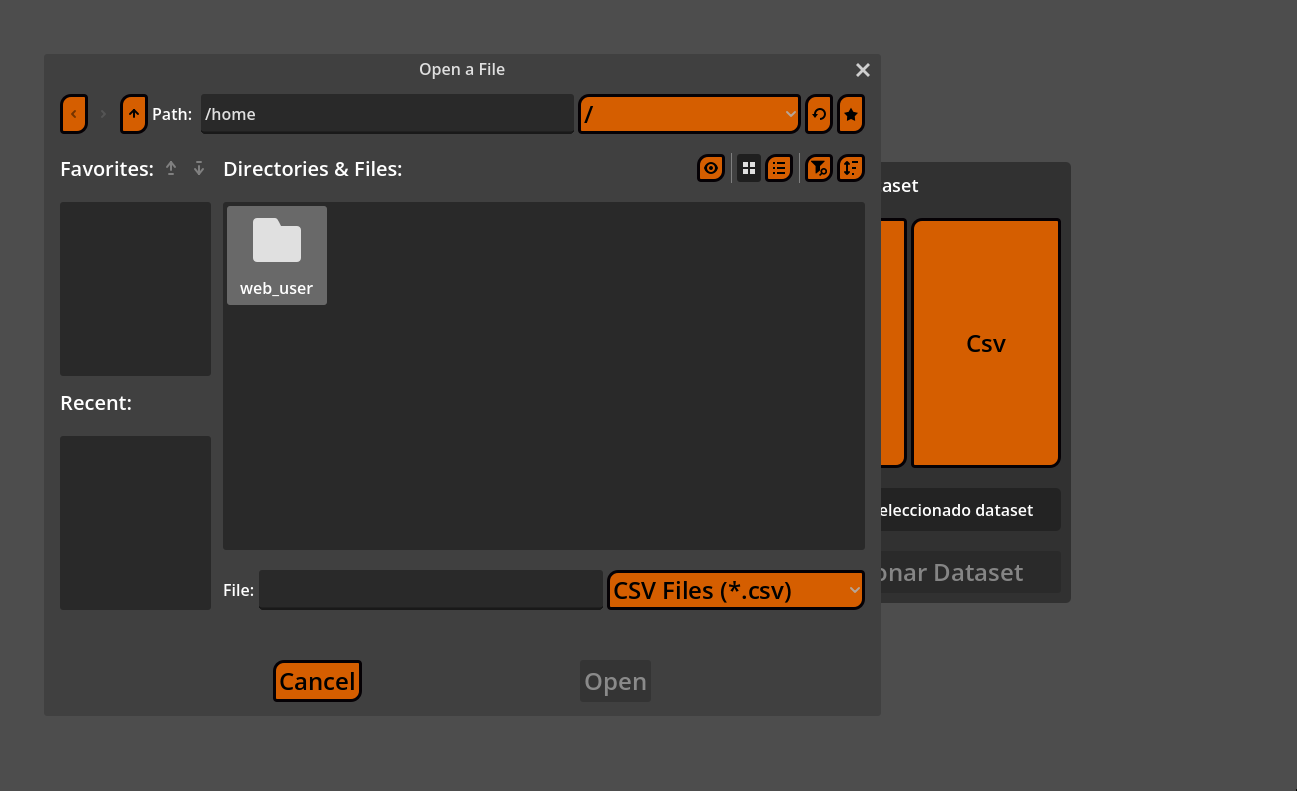
\includegraphics[width=0.7\textwidth]{imaxes/a_menugodot.png}
  \caption{Imagen del menú nativo de Godot que se abría en la versión web antes de crear el puente de JavaScript.}
  %\label{fig:}
\end{figure}

%\include{anexos/...}

 \printglossary[type=\acronymtype,title=\nomeglosarioacronimos]
 \printglossary[title=\nomeglosariotermos]

 \bibliographystyle{IEEEtranN}
 \bibliography{\bibconfig,bibliografia/bibliografia}
 \clearpage
 
\end{document}

%%%%%%%%%%%%%%%%%%%%%%%%%%%%%%%%%%%%%%%%%%%%%%%%%%%%%%%%%%%%%%%%%%%%%%%%%%%%%%%%
